\documentclass[%
  aspectratio=169,
  9pt,
  USenglish,
  titlegraphic, % store custom image to .images/titlegraphic
  affiliationintitlepagehead,
  %progressbar,
  affiliation,
]{beamer}

\usetheme{TUM}

\input{preamble.tex}


\usetikzlibrary{external}
\tikzexternalize[prefix=tikz/]
\tikzexternalize
\tikzexternaldisable

\usepackage{tummath}

\setbeamertemplate{blocks}[rounded][shadow=false]

%	\end{itemize}
%	
%	Research Scope 
%	\begin{itemize}
%		\item Imbalance of Raster and Label Data
%		\item Analogies to NLP
%		\item Sequence modeling
%	\end{itemize}
%		
%	Research Projects
%	\begin{itemize}
%		\item Crop Classification with Multi-temporal Land Cover Classification
%		\item Early Classificaiton of Time Series
%	\end{itemize}
%		
%		
%\end{frame}


\title{Earth Observation and Machine Learning}
\subtitle{From Language Model to Earth Model}
\author[M. Rußwurm]{Marc Rußwurm M.Sc., advised by Dr. Marco Körner}
\institute[TUM]{Technical University of Munich, Germany\\
	Remote Sensing Technology}
\date{May 3rd 2019, OATML-Lab, Oxford, UK}

\begin{document}

\begin{frame}[t]
\titlepage
\end{frame}


{\setbeamercolor{background canvas}{bg=white}
	\begin{frame}[plain]
	\vfill
	\begin{center}
		\Huge\color{tumgraydark}
		About
		\hspace{2em}\includegraphics[width=5cm]{images/marc}
	\end{center}
	\vfill
\end{frame}
}


%%
%\begin{frame}
%	\frametitle{Marc Rußwurm}
%	
%	\begin{columns}
%		\column{.66\textwidth}
%			\uncover<2->{
%				\begin{itemize}
%					\item born in raised in Bavaria, Germany.
%					\item recently finished Master Geodesy \& Geoinformation @ TU Munich
%					\item now started PhD @ TUM/DLR \\ Chair of Remote Sensing Technology
%					\item member Computer Vision Research Group of the Chair
%				\end{itemize}
%			}
%			\uncover<3->{
%				\vspace{1em}
%				scientific interests
%				\begin{itemize}
%					\item multi-temporal EO
%					\item time series with Recurrent Nets
%					\item natural language processing $\rightarrow$ EO
%				\end{itemize}
%			}
%			\column{.33\textwidth}
%			
%			\includegraphics[width=\textwidth]{images/marc}
%%			\begin{tikzpicture}
%%			
%%			\node(marc) at (0,0){};
%%			
%%			\end{tikzpicture}
%		
%	\end{columns}
%\end{frame}

\begin{frame}
\frametitle{Background}

\begin{columns}
	\column{.75\textwidth}
%	Marc Rußwurm
%	\uncover<2->{
%		\begin{itemize}
%			\item born in raised in Bavaria, Germany.
%%			\item recently finished Master Geodesy \& Geoinformation @ TU Munich
%%			\item now started PhD @ TUM/DLR \\ Chair of Remote Sensing Technology
%%			\item member Computer Vision Research Group of my Chair
%		\end{itemize}
%	}
%	\uncover<3->{
%		\vspace{1em}
%		scientific interests
%		\begin{itemize}
%			\item multi-temporal EO
%%			\item time series with Recurrent Nets
%%			\item natural language processing $\rightarrow$ EO
%		\end{itemize}
%	}
%	\column{.25\textwidth}
%	\begin{tikzpicture}
%	
%	\node(marc) at (0,0){\includegraphics[width=\textwidth]{images/marc}};
%	
%	\end{tikzpicture}
	
\end{columns}

\tikzstyle{event} = [font=\small, text width=3.8cm, rounded corners=2em, inner sep=.7em]
\tikzstyle{date} = [font=\small, fill=white]
%
%\vspace{2em}

\begin{tikzpicture}[xscale=9, yscale=.85]

	\visible<1->{\node[anchor=east, label=Earth Observation] at (0,0){\includegraphics[width=3cm]{images/dscovrepic/epicw1}};}
	\visible<4->{\node[anchor=west, label=Machine Learning] at (1.1,0){\lfcn{.75}};}

	\node[event, fill=tumorange!50] at (.2,1) {2012-2018 \\ \textbf{Bachelor/Master} \\ Geodesy and Geoinformation};
	
	\visible<2->{\node[event, fill=tumbluelight] at (.3,-1) {2014 \\ Interned at University of Otago, NZ. \\ Geodata Visualization};}
	
	\visible<3->{\node[event, fill=tumbluelight] at (.1,-3) {2016 \\ Erasmus-interned at Polish Earth Observation Center \\ \textbf{Opium Poppy Detection}};}
	
	\visible<4->{\node[event, fill=tumorange!50] at (.7,2) {2018-2022 \\ \textbf{PhD} with Supervisor from Computer Vision \\ Multi-temporal Earth Observation};}
	
	\visible<5->{\node[event, fill=tumbluelight] at (.7,-3) {2018 \\ Participant \\ Frontier Developments Lab \\ Disaster Relief with \textbf{CNN data fusion}};}
	
	\visible<6->{\node[event, fill=tumbluelight] at (.8,-.5) {2019 \\ Research Stay IRISA Obelix Lab in France \\ \textbf{Early Classification of Time Series}};}
	
	
%	\draw (.8,6) node[date, above]{2019} -- node[event]{Research Stay \\ IRISA Obelix Lab in France} (.8,-3);
	
%	\draw (0,0)  node[left]{Earth Observation} -- node[at end, right]{Machine Learning} (1,0);
%	
%	\draw (.2,1) node[date, above]{2012-2018} -- node[event]{Studied B.Sc M.Sc Geodesy and Geoinformation} (.2,-1);
%
%	\draw (.2,2) node[date, above]{2014} -- node[event]{Interned at University of Otago, NZ. Geodata Visualization} (.2,-1);
%	
%	\draw (.1,3) node[date, above]{2016} -- node[event]{Erasmus-interned at Polish Earth Observation Center} (.1,-2);
%	
%	\draw (.7,4) node[date, above]{2018-2022} -- node[event]{PhD Supervisor in Computer Vision} (.7,-3);
%	
%	\draw (.6,5) node[date, above]{2018} -- node[event]{Participant in Frontier Developments Lab} (.6,-3);
%	 
%	\draw (.8,6) node[date, above]{2019} -- node[event]{Research Stay at IRISA Obelix Lab in France} (.8,-3);
	 
\end{tikzpicture}

\end{frame}



\newcommand{\focusdata}{{\color{tumblue}\textbf{data}~}}
\newcommand{\focusmethod}{{\color{tumorange}\textbf{method}~}}



\begin{frame}
	\frametitle{This Talk}
	
	\Large
	
	Organized in three parts
	
	\begin{description}
		\item[Part I] Overview Earth Observation
		\item[Part II] Research and Projects
		\item[Part III] Workshops and Programs around EO and ML
	\end{description}
\end{frame}

%{\setbeamercolor{background canvas}{bg=tumblue}
%	\begin{frame}[plain]
%	\vfill
%	\begin{center}
%		\Huge\color{tumwhite}
%		Remote Sensing Technology
%		\includegraphics[width=5cm]{images/TUM-white}
%	\end{center}
%	
%	\vfill
%\end{frame}
%}







{\setbeamercolor{background canvas}{bg=black}
	\begin{frame}[plain]
	
		\vfill
		\Huge\color{white}
		\begin{center}
			\begin{columns}
				\column{.5\textwidth}
				\vspace{7em}
				
				\hfill 
				Part I: Earth Observation
				\column{.5\textwidth}
				
				\includegraphics[width=5cm]{images/dscovrepic/epic1}
				%\includegraphics[width=7cm]{images/fdl}
			\end{columns}
		\end{center}
		
		\vfill
	\end{frame}
}






%{\setbeamercolor{background canvas}{bg=tumblue}
%\begin{frame}[plain]
%\vfill
%\begin{center}
%\Huge\color{tumwhite}
%Supervised Crop Type Mapping
%\includegraphics[width=5cm]{images/TUM-white}
%\end{center}
%
%\vfill
%\end{frame}
%}

%\begin{frame}
%\frametitle{The Team}
%
%Image of the people in the Chair
%\end{frame}

%\begin{frame}
%	\newcommand{\bblock}[6]{
	\draw[#1] (axis cs: #2,#4) rectangle node[text=white]{#6} (axis cs: #3,#5);
}

\newcommand{\event}[2]{
	\draw[draw=tumblue] (axis cs: #1,0) -- (axis cs: #1,8) node[above,font=\small]{#2};
}

\begin{tikzpicture}
\tikzstyle{project}=[fill=tumblue, draw=none, font=\tiny]
\tikzstyle{phase}=[fill=tumgray, draw=none, font=\small]
\tikzstyle{futureproject}=[fill=tumblue, draw=none, font=\tiny, fill opacity=0.2]
\tikzstyle{conference}=[fill=tumorange, draw=none, very thick, font=\tiny]

\begin{axis}[
	date coordinates in=x,
	xticklabel=\year,
	xtick={2019-01-01,2020-01-01,2021-01-01},
	width=\textwidth,
	height=6cm,
	ymax=10,
	ymin=-5,
	xmin=2018-05-01,
	xmax=2021-09-01,
	hide y axis,
	axis line style={draw=none}]
	
	\event{2018-06-01}{start}
	\bblock{project}{2018-06-25}{2018-08-17}{1}{2}{FDL}
	\bblock{project}{2018-10-01}{2019-2-15}{2}{3}{IRISA Obelix}
%	\block{conference}{2018-12-01}{2018-12-06}{4}{5}{NeurIPS}
%	\block{conference}{2018-11-12}{2018-11-16}{5}{6}{$\Phi$-week}
%	\block{conference}{2019-01-27}{2019-02-01}{5}{6}{AAAI}
	\event{2019-02-10}{this exposé}
	\bblock{project}{2019-3-01}{2019-10-01}{3}{4}{crop type mapping}
	%\block{project}{2019-8-01}{2019-10-15}{2}{3}{ESA}
	\bblock{futureproject}{2019-10-01}{2020-06-01}{4}{5}{biomass and crop yield}
	\bblock{futureproject}{2020-06-01}{2020-12-31}{5}{6}{nowcasting of atmospheric effects}
	\bblock{futureproject}{2021-01-01}{2021-06-01}{6}{7}{writing}
	\event{2021-06-01}{defense}
	
	\draw[left color=tumbluelight, right color=tumbluedark, draw=none, fill opacity=0.2] (axis cs: 2018-06-01,-2) rectangle node[left=10em, font=\small]{supervised} node[text=white, font=\small]{semi-supervised} node[right=9em, text=white, font=\small]{unsupervised} (axis cs: 2021-06-01,-1);
	
	\bblock{phase}{2018-06-01}{2018-11-31}{-4}{-3}{warm-up}
	\bblock{phase}{2019-02-01}{2020-11-31}{-4}{-3}{research}
	\bblock{phase}{2021-02-01}{2021-06-01}{-4}{-3}{wrap-up}
	
%\addplot [red] expression {1/(1+exp(-x))};  % <-- fails if uncommented
\end{axis}
\end{tikzpicture}

%\end{frame}
%
%\begin{frame}
%	\setrand{0}{100}{0.01}{1}
	\newcommand{\drawmatrix}{
		\left(\begin{matrix}\nextrand\thisrand\\\nextrand\thisrand\\\nextrand\thisrand\end{matrix}\right)
	}

	\newcommand{\image}[1]{
		\begin{tikzpicture}
			\node(img){\includegraphics[width=2cm]{#1}};
			\node[minimum width=.5em,minimum height=.5em, fill=tumbluelight, xshift=-1em] at (img)(rect){};
			
			\node[right=of rect, fill=tumbluelight,, inner sep=.2em, rounded corners=1em,  opacity=.2](m){$\drawmatrix$};
			\draw[tumbluelight] (rect.north) -- (m.north);
			\draw[tumbluelight] (rect.south) -- (m.south);
		\end{tikzpicture}
	}

	
	\begin{tikzpicture}[node distance=1em]
		\node[font=\scriptsize](e1){\image{images/analogy_examples/170127_snow.png}};
		\node[right=of e1, font=\scriptsize](e2){\image{images/analogy_examples/160929_clear.png}};
		\node[right=of e2, font=\scriptsize](e3){\image{images/analogy_examples/161115_cloudy.png}};
		\node[right=of e3, font=\scriptsize](e4){\image{images/analogy_examples/160728_partlycloudy.png}};
		
		\node[below=of e1, font=\scriptsize](t1){$E(\text{\textbf{The}})=\drawmatrix$};
		\node[below=of e2, font=\scriptsize](t2){$E(\text{\textbf{eagle}})=\drawmatrix$};
		\node[below=of e3, font=\scriptsize](t3){$E(\text{\textbf{has}})=\drawmatrix$};
		\node[below=of e4, font=\scriptsize](t4){$E(\text{\textbf{landed}})=\drawmatrix$};
		
		\node[above=of e1](x1){$\V{x}_1$};
		\node[above=of e2](x2){$\V{x}_2$};
		\node[above=of e3](x3){$\V{x}_3$};
		\node[above=of e4](x4){$\V{x}_4$};
		
		\node[right= 7em of e4](eo){$f(\M{X})$};
		\node[right= 7em of t4](nlp){$f(\M{X})$};
		
		\draw[-stealth] (e4) -- node[midway,above]{EO model} (eo);
		\draw[-stealth] (t4) -- node[midway,above]{NLP model} (nlp);
	\end{tikzpicture}
%\end{frame}

%
%{\setbeamercolor{background canvas}{bg=black}
%	\begin{frame}[plain]
%	\vfill
%	\begin{center}
%		\Huge\color{tumwhite}
%		Earth Observation Data $\M{X}$
%		\includegraphics[width=5cm]{images/dscovrepic/epic1}
%	\end{center}
%	
%	\vfill
%\end{frame}
%}


\begin{frame}
	\frametitle{System Earth}
	
	\begin{columns}

	\column{.5\textwidth}
	
	{
%		The Earth is a complex system.
%		Only some components is observable by 
%		\begin{itemize}
%			\item satellite-based or
%			\item in-situ observations
%		\end{itemize}
%		
		
%	\begin{equation*}\V{y} = f({\M{X}})\end{equation*}
%	partially observe the complex system Earth
	\textbf{Partially measuring} System Earth
	{\Huge
		\begin{equation*}
			\M{X} = \sat\left({\earth}\right)
		\end{equation*}
	}

	\vspace{1em}
	\textbf{knowledge extraction} through pattern recognition and machine learning
	
	{\Huge\begin{equation*}\V{?} = f({\M{X}})\end{equation*}}
	}

	\column{.5\textwidth}
	
	\begin{tikzpicture}[xscale=3, yscale=2]
		\node(earth) at (0,0) {\includegraphics[width=7cm]{images/dscovrepic/epicw1}};	

	\end{tikzpicture}
	
	
	\end{columns}

%	\includegraphics[width=5cm]{images/Earth_gravity}
%	\includegraphics[width=5cm]{images/dscovrepic/epicw1}
%	\includegraphics[width=5cm]{images/earthnullschool/sealevelpressure}
%	\includegraphics[width=5cm]{images/earthnullschool/misery_index}
%	\includegraphics[width=5cm]{images/earthnullschool/temp}
%	\includegraphics[width=5cm]{images/dscovrepic/epicw1}
	\end{frame}
%
%\begin{frame}
%	\frametitle{Measurements}
%	
%	\begin{columns}
%	
%	\columnwidth{.5\textwidth}
%	In-Situ Measurements
%	\begin{itemize}
%		\item Seismographs
%		\item Flux-Towers
%		\item Weather Stations
%		\item GNSS ground station
%		\item ...
%	\end{itemize}
%
%	Satellite-based Sensors
%	\begin{itemize}
%		\item Gravimetry
%		\item GNSS Science
%		\item Atmospheric Sciences
%		\item Radar (Active Sensors)
%		\item Optical Satellite Sensors
%	\end{itemize}
%
%	\columnwidth{.5\textwidth}
%
%	\begin{tikzpicture}
%		content...
%	\end{tikzpicture}
%
%	\end{columns}
%
%\end{frame}

%
\begin{frame}
\frametitle{Passive Optical Sensors}
\begin{columns}
	\column{.5\textwidth}
	
	
	\begin{itemize}[itemsep=.5em]
		\item<1-> Sensor measures \textbf{Digital Numbers} $\text{DN}(\lambda)$ for each band wavelength $\lambda$. 
		\item<2-> \textbf{Digital Numbers} are normalized to \textbf{Radiance} 
		$L(\lambda), \left[\frac{W}{\text{sr}m^1}\right]$ by gain and offset calibration.
		\item<4-> Radiance is normalized to \textbf{top-of-atmosphere reflectance} $\rho(\lambda)$
		\item<4-> \textbf{Bottom-of-atmosphere reflectances} are reconstructed using a functional model of the atmosphere.
	\end{itemize}
	
%	Radiance $R_\lambda$ from measured Digital Numbers via calibrated gain $\alpha$ and offset $\beta$
%	\begin{equation*}
%		L_\lambda = \alpha \text{DN}_\lambda + \beta, \left[\frac{W}{\text{sr}m^1}\right]
%	\end{equation*}
%	
%	top-of-atmosphere reflectance $\rho_\lambda$ as normalized Radiance $R_\lambda$ with solar 
%	\begin{equation*}
%	\rho_\lambda = \frac{L_\lambda}{\cos(\varphi_\text{sun})}
%	\frac{
%		\pi d^2
%	}
%	{
%		E_\text{sun}(\lambda)
%	}
%	\end{equation*}
%	
%	\vspace{1em}
%	
%	\begin{itemize}
%		\item measured radiance $L(\lambda)$
%		\item solar irradiance $E_\text{sun}(\lambda)$
%		\item solar zenith angle $\varphi_\text{sun}$
%		\item squared Earth-Sun distance $d$ in AU
%	\end{itemize}

	
	\column{.5\textwidth}
	
	
	\begin{tikzpicture}
	
	
	%	\draw [black,dotted, fill=tumbluelight,domain=110:70] plot ({13*cos(\x)}, {13*sin(\x)-12.8});
	\draw [fill=tumivory,domain=110:70] plot ({10*cos(\x)}, {10*sin(\x)-10});
%	\draw [fill=tumbluelight,domain=110:70] plot ({12*cos(\x)}f, {12*sin(\x)-10});
	
	
	\node(sun) at (-2,2) {\includegraphics[width=10mm]{images/icons/sun}};
	\node[rotate=130,anchor=center](sat) at (2,2) {\includegraphics[width=10mm]{images/icons/sat2}};
	
	\node(px) at ({10*cos(90)}, {10*sin(90)-10.1}){
		\begin{tikzpicture}[xscale=.5,yscale=.25]
		\draw[fill=tumbluelight] (0,0) -- (1,0) -- (2,1) -- (1,1) -- (0,0);
		\end{tikzpicture}
		%\includegraphics[width=5mm]{images/icons/house}
	};
	
	\draw[-stealth] (sun) -- node[midway,sloped]{\wave} (px);
	\draw[-stealth] (px) -- node[midway,sloped]{\wave} (sat);
	
	\visible<3->{\draw[-stealth] (sun) -- node[midway,sloped]{\wave} (sat);
	\draw[draw=tumgray] (px) -- node[at end,left]{$\varphi_\text{sun}$} ++(0,1.4); 
	\draw [draw=tumgray, domain=130:90] plot ({1*cos(\x)}, {1*sin(\x)});
	}
	
	\node[above=.5em of sun]{$E_\text{sun}(\lambda)$};
	\visible<1>{\node[above=4em of sat]{$DN(\lambda)$};}
	\visible<2>{\node[above=4em of sat]{$L(\lambda)$};}
	\visible<3>{\node[above=4em of sat]{$\rho_\text{toa}(\lambda)$};}
	\visible<4>{\node[above=4em of sat]{$\rho_\text{boa}(\lambda)$};}

	%		\draw[red] (0,0) sin (1,2);
	
	\end{tikzpicture}
	
\end{columns}

\end{frame}

\newcommand{\rastergrid}{
	\begin{tikzpicture}
	% each layer
	\begin{scope}[scale=2]
	
	% raster size
	\def\d{0.7}		
	
	% distance layer
	\def\s{\d*5}
	
	\foreach \i in {1,...,6}
	{		
		\begin{scope}[
		yshift=\s*\i,every node/.append style={
			yslant=0.5,xslant=-1},yslant=0.5,xslant=-1
		]
		%\draw[step=3.33mm] (0,0) grid (1,1);
		%\fill[black,fill opacity=.9] (0.333,0.333) rectangle (0.333,0.333);    	    	  
		
		\foreach \row in {0,...,2}{
			\foreach \col in {0,...,2}{
				\draw[tumblack, fill=tumblue!\pdfuniformdeviate 40,fill opacity=1,rounded corners=1] (\col*\d/3,\row*\d/3) rectangle (\col*\d/3+\d/3, \row*\d/3+\d/3);
				%                 \draw[black, fill=black!\pdfuniformdeviate 40,fill opacity=1,rounded corners=1] (\col*\d/3,\row*\d/3) rectangle (\col*\d/3+\d/3, \row*\d/3+\d/3);
			}
		}
		
		%\draw[step=3.33mm] (0,0) grid (1,1);
		%\fill[white,fill opacity=.9] (0,0) rectangle (1,1);
		\end{scope}
	}
	\end{scope}
	\end{tikzpicture}
}


%\begin{frame}
%\frametitle{Spectral Band}
%\end{frame}


\newcommand{\myvec}[1]{\ensuremath{\begin{pmatrix}#1\end{pmatrix}}}
\begin{frame}
\frametitle{Spatial and Temporal Discretization}

\begin{columns}
	\column{.5\textwidth}
	
	{
		\begin{equation*}
		\M{X} = \myvec{\rho_{\lambda_1} \\ \rho_{\lambda_2} \\ \dots \\ \rho_{\lambda_n}}
		\end{equation*}
	}
	
	
	
	Spectral reflectance of \textbf{spectral bands} disctretized on a \textbf{spatial grid}. Each grid cell is georeferenced by its Longitude $\Lambda$ and Latitude $\Phi$.
	Acquisitions in regular \textbf{temporal intervals}.
	
	\column{.5\textwidth}
	
	
	
	\begin{tikzpicture}
	
	%	\node(a){\includegraphics[width=3cm]{images/s2grid/1}};
	
	%	\draw[step=1cm,gray,very thin] (-2,-2) grid (6,6);
	
	
	\draw [fill=tumivory,domain=110:70] plot ({11*cos(\x)}, {11*sin(\x)-8.5});
	
	\begin{scope}[scale=1]
	
	% raster size
	\def\d{1}		
	
	% distance layer
	\def\s{\d*50}
	
	\node at (-1.7,2.4){$t_{i-1}$};
	\node at (-1.7,4.2){$t_i$};
	\node at (-1.7,6){$t_{i-1}$};
	
	\node at (1,1.9){$\Lambda$};
	\node at (-1,1.9){$\Phi$};
	
	%		\draw[step=1.0,black,thin] (-2,0) grid (2,5);
	
	
	\foreach \i in {1,...,3}
	{		
		
		\begin{scope}[
		yshift=\s*\i,every node/.append style={
			yslant=0.5,xslant=-1},yslant=0.5,xslant=-1,scale=0.35
		]
		%\draw[step=3.33mm] (0,0) grid (1,1);
		%\fill[black,fill opacity=.9] (0.333,0.333) rectangle (0.333,0.333);    	    	  
		
		
		
		\foreach \row in {0,...,3}{
			\foreach \col in {0,...,3}{
				\draw[tumblack, fill=tumblue!\pdfuniformdeviate 40,fill opacity=1,rounded corners=1] (\col,\row) rectangle (\col+1, \row+1);
				
				\node[font=\tiny, text=tumblue] at (\col + 0.5,\row + 0.5) {$\V{x}$};
				
				%                 \draw[black, fill=black!\pdfuniformdeviate 40,fill opacity=1,rounded corners=1] (\col*\d/3,\row*\d/3) rectangle (\col*\d/3+\d/3, \row*\d/3+\d/3);
			}
		}
		
		%\draw[step=3.33mm] (0,0) grid (1,1);
		%\fill[white,fill opacity=.9] (0,0) rectangle (1,1);
		\end{scope}
	}
	\end{scope}
	
	
	
	\end{tikzpicture}
	
\end{columns}


%	\begin{equation*}
%		x_{geo} = \begin{pmatrix} \Lambda \\ \Phi\end{pmatrix} + x_{image} \begin{pmatrix}px_w & 0 \\ 0 & px_h\end{pmatrix}
%	\end{equation*}

\end{frame}


\begin{frame}

\vfill
\Huge\color{black}
\begin{center}
	\begin{columns}
		\column{\textwidth}
		\vspace{7em}
		
		\textbf{Hands-on:}
		\hfill 
		Optical Earth Observation
		%			\includegraphics[width=5cm]{images/dscovrepic/epic1}
		%\includegraphics[width=7cm]{images/fdl}
	\end{columns}
\end{center}

\vfill

\end{frame}


%
%\end{document}




{	
%	\setbeamercolor*{Title bar}           {bg=tumblack,fg=tumblue}
%	\setbeamercolor*{Location bar}        {bg=tumblack,fg=tumblue}
%	\setbeamercolor*{frametitle}          {parent=Title bar}
%	\setbeamercolor*{normal text}         {bg=tumblack,fg=tumwhite}
%	
	
\tikzstyle{dist} = [font=\tiny]
	
\begin{frame}
  \frametitle{Weather Satellites}
  \framesubtitle{At the Langrange 1 Point}
  
  
  
  
  \begin{columns}
  	\column{.3\textwidth}
  	
  	\hspace{2em}\textbf{dscovr:epic}
  	\begin{itemize}
  		\item 8 km spatial resolution
  		\item image every 20s
  		\item 10 spectral channels
  	\end{itemize}
  	
  	\column{.3\textwidth}
  	\hspace{2em}
  	\begin{tikzpicture}
  	
  	
  	
  	\visible<1>{\node[rotate=-20, anchor=center](earth) at (0,0) {\includegraphics[width=5mm]{images/icons/earth}};}
  	\visible<2>{\node[rotate=0, anchor=center](earth) at (0,0) {\includegraphics[width=5mm]{images/icons/earth}};}
  	\visible<3>{\node[rotate=20, anchor=center](earth) at (0,0) {\includegraphics[width=5mm]{images/icons/earth}};}
  	\visible<4>{\node[rotate=40, anchor=center](earth) at (0,0) {\includegraphics[width=5mm]{images/icons/earth}};}
  	
  	\only<4>{\node at (-.2,-1) {\includegraphics[width=3mm]{images/icons/moon}};};
  	
  	\node[anchor=center](sat) at (0,-2) {\includegraphics[width=5mm]{images/icons/sat2}};
  	\node at (0,-4) {\includegraphics[width=5mm]{images/icons/sun}};
  	
  	\draw[dist] (earth) -- node[midway,below,sloped]{1.5 Mio km} (sat);
  	
  	\node[left=1em of sat, text=white]{$L_1$};
%  	\draw [red,thick,domain=230:315] plot ({2*cos(\x)}, {2*sin(\x)});
  	\end{tikzpicture}
  	
  	\column{.7\textwidth}
  	
  	\only<1>{\includegraphics[width=6cm]{images/dscovrepic/epicw1}}
  	\only<2>{\includegraphics[width=6cm]{images/dscovrepic/epicw2}}
  	\only<3>{\includegraphics[width=6cm]{images/dscovrepic/epicw3}}
  	\only<4>{\includegraphics[width=6cm]{images/dscovrepic/epicwl2}}

\end{columns}

\url{twitter.com/dscovr_epic}
\url{epic.gsfc.nasa.gov}

\hfill
\vfill
\scriptsize Icons from \url{https://www.flaticon.com}
 \end{frame}

\begin{frame}
\frametitle{Weather Satellites}
\framesubtitle{At geostationary orbit}


\begin{columns}
	\column{.3\textwidth}
	
	\hspace{2em}\textbf{MeteoSAT, GOES}
	\begin{itemize}
		\item 2.5 - 5km km spatial resolution
		\item image every 15 minutes
		\item 12 spectral 0channels
	\end{itemize}
	
	
	\column{.3\textwidth}
%	\hspace{2em}
	\begin{tikzpicture}
	
	
	\draw [tumgraylight,dotted,domain=230:315] plot ({2*cos(\x)}, {2*sin(\x)});
	
	\visible<1>{
	\node[rotate=-20, anchor=center](earth) at (0,0) {\includegraphics[width=5mm]{images/icons/earth}};
	\node[anchor=center, rotate around={-20:(0,2)}](sat) at (0,-2) {\includegraphics[width=5mm]{images/icons/sat2}};
	\draw[dist] (earth) -- node[midway,below,sloped]{35k km} (sat);
	}
	\visible<2>{
	\node[rotate=0, anchor=center] at (0,0) {\includegraphics[width=5mm]{images/icons/earth}};
	\node[anchor=center, rotate around={0:(0,2)}](sat) at (0,-2) {\includegraphics[width=5mm]{images/icons/sat2}};
	\draw[dist] (earth) -- node[midway,below,sloped]{35k km} (sat);}
	\visible<3>{
	\node[rotate=20, anchor=center] at (0,0) {\includegraphics[width=5mm]{images/icons/earth}};
	\node[anchor=center, rotate around={20:(0,2)}](sat) at (0,-2) {\includegraphics[width=5mm]{images/icons/sat2}};
	\draw[dist] (earth) -- node[midway,below,sloped]{35k km} (sat);
	}
%	\visible<4>{
%	\node[rotate=40, anchor=center] at (0,0) {\includegraphics[width=5mm]{images/icons/earth}};
%	\node[anchor=center, rotate around={40:(0,2)}](sat) at (0,-2) {\includegraphics[width=5mm]{images/icons/sat2}};
%	\draw (earth) -- (sat);
%}




	\node at (0,-4) {\includegraphics[width=5mm]{images/icons/sun}};
	
	\node at (-.2,-3) {\includegraphics[width=3mm]{images/icons/moon}};
	
	\end{tikzpicture}
	
	\column{.6\textwidth}
	
	\only<1>{\includegraphics[width=6cm]{images/EUMETSAT/MET10_RGBNatColourEnhncd_CentralEurope_20190405090000}}
	\only<2>{\includegraphics[width=6cm]{images/EUMETSAT/MET10_RGBNatColourEnhncd_CentralEurope_20190405100000}}
	\only<3>{\includegraphics[width=6cm]{images/EUMETSAT/MET10_RGBNatColourEnhncd_CentralEurope_20190405110000}}
%	\only<4>{\includegraphics[width=6cm]{images/EUMETSAT/MET10_RGBNatColourEnhncd_CentralEurope_20190405120000}}
	
\end{columns}

\url{http://oiswww.eumetsat.org}
\hfill
\vfill
\scriptsize Icons from \url{https://www.flaticon.com}
\end{frame}
}

\begin{frame}
	\frametitle{Sun Synchronus Orbit}
	\begin{columns}
		\column{.66\textwidth}
		
%		Orbiting closer capture less area with higher spatial resolution.
%		The comparatively large earth Shadow forces these satellites on the sun synchornous orbit
		
		\textbf{Environmental Satellites} with 1km spatial resolution every day
		\begin{itemize}
			\item NASA's MODIS Aqua/Terra
			\item ESA's Sentinel 3
		\end{itemize}
		\vspace{2em}
		 
		\textbf{Multi-spectral satellites} with 10-60m spatial resolution 3-10 days
		\begin{itemize}
			\item NASA's Landsat Satellites (since 70s!)
			\item ESA's Sentinel 2
		\end{itemize}
		 
%		\begin{itemize}
%			\item 
%			\item 
%		\end{itemize}
		
		\column{.33\textwidth}
		
			\only<1-3>{
			\begin{tikzpicture}
			
			
			\draw [tumgraylight,dotted,domain=230:315] plot ({2*cos(\x)}, {2*sin(\x)});
			
			\visible<1>{
				\node[rotate=0, anchor=center](earth) at (0,0) {\includegraphics[width=20mm]{images/icons/earth}};
				\node[anchor=center, rotate around={-20:(0,2)}](sat) at (0,-2) {\includegraphics[width=5mm]{images/icons/sat2}};
				\draw[font=\tiny] (earth) -- node[midway,below,sloped]{800km} (sat);
			}
			\visible<2>{
				\node[rotate=0, anchor=center](earth) at (0,0) {\includegraphics[width=20mm]{images/icons/earth}};
				\node[anchor=center, rotate around={0:(0,2)}](sat) at (0,-2) {\includegraphics[width=5mm]{images/icons/sat2}};
				\draw[font=\tiny] (earth) -- node[midway,below,sloped]{800km} (sat);
			}
			\visible<3>{
				\node[rotate=0, anchor=center](earth) at (0,0) {\includegraphics[width=20mm]{images/icons/earth}};
				\node[anchor=center, rotate around={20:(0,2)}](sat) at (0,-2) {\includegraphics[width=5mm]{images/icons/sat2}};
				\draw[font=\tiny] (earth) -- node[midway,below,sloped]{800km} (sat);
			}
			\end{tikzpicture}
			}
%			
%			\only<4>{
%				\includegraphics[width=5cm]{images/sso_white}
%			}
		
%			\includegraphics[width=.33\textwidth]{images/sso_white}
		
	\end{columns}
%	
%	image from \url{https://en.wikipedia.org/wiki/Sun-synchronous_orbit}
\end{frame}

\begin{frame}
	\frametitle{Global Environmental Satellites}
	
	\begin{columns}
		\column{.5\textwidth}
		
		Moderate Resolution Spectrometer
		\begin{itemize}
			\item images every day
			\item resolution $\approx 1km$
			\item $> 50$ spectral bands
		\end{itemize}
		
		\column{.5\textwidth}
		
		\includegraphics[width=\textwidth]{images/modis}
		
	\end{columns}
	
	\url{https://worldview.earthdata.nasa.gov/}
	
\end{frame}

\begin{frame}
	\frametitle{Multi Spectral Satellites -- Example Sentinel 2 or Landsat}
	
	\begin{columns}[t]
		
		\column{.5\textwidth}
		
		
		
		\textbf{USGS Landsat}
		\begin{itemize}
			\item spatial resolution 30m
			\item covers every point on Earth every 16 days
			\item 11 spectral bands
			\item since the 80s
		\end{itemize}
		
		\vspace{2em}
		
		\textbf{ESA Sentinel-2}
		\begin{itemize}
			\item spatial resolution 10m-60m
			\item covers every point on Earth every 2-5 days
			\item 13 spectral bands
			\item since 2016
		\end{itemize}
		
		\column{.5\textwidth}
		
		\includegraphics[width=\textwidth]{images/airbus_Sentinel-2_022415_945}
		
		©AIRBUS DEFENCE AND SPACE
	\end{columns}
	
	
	
\end{frame}

\begin{frame}
\frametitle{Multi Spectral Satellites -- Example Sentinel 2}

%\newcommand{\focusband}[1]{\color{tumorange} #1}

\begin{columns}
	\column{.33\textwidth}
%	
%	\color{tumgray}
	\only<1>{True Color}
	\only<2>{False Color}
	\only<3>{False Color Urban}
	\only<4>{Short-Wave Infra Red Bands}
	\only<5>{MoistureIndex}
	\only<6>{Vegetation Index (NDVI)}
	\only<7>{Water Index (NDWI)}
	
	\small
	\begin{equation*}
	\M{X} = \begin{pmatrix}
		\rho_{B1} \\ 
		\only<2,3,4,5,6,7>{\rho_{B2}} \only<1>{\color{tumorange}\rho_{B2}} \\
		\only<3,4,5,6>{\rho_{B3}} \only<1,2,7>{\color{tumorange}\rho_{B3}} \\
		\only<5,7>{\rho_{B4}} \only<1,2,3,4,6>{\color{tumorange}\rho_{B4}} \\
		\rho_{B5} \\
		\rho_{B6} \\
		\rho_{B7} \\
		\only<1,3,4,5>{\rho_{B8}} \only<2,6,7>{\color{tumorange}\rho_{B8}} \\
		\only<1,2,3,6,7>{\rho_{B8A}} \only<4,5>{\color{tumorange}\rho_{B8A}} \\
		\rho_{B9} \\
		\rho_{B10} \\
		\only<1,2,4,6,7>{\rho_{B11}} \only<3,5>{\color{tumorange}\rho_{B11}} \\
		\only<1,2,5,6,7>{\rho_{B12}} \only<3,4>{\color{tumorange}\rho_{B12}}
		\end{pmatrix} \xrightarrow{visualize} 
		\begin{pmatrix}
			\only<1>{\rho_{B4} \\ \rho_{B3} \\ \rho_{B2}}
			\only<2>{\rho_{B8} \\ \rho_{B4} \\ \rho_{B3}}
			\only<3>{\rho_{B12} \\ \rho_{B11} \\ \rho_{B4}}
			\only<4>{\rho_{B12} \\ \rho_{B8A} \\ \rho_{B4}}
			\only<5>{\frac{\rho_{B8A}-\rho_{B11}}{\rho_{B8A}+\rho_{B11}}}
			\only<6>{\frac{\rho_{B8}-\rho_{B4}}{\rho_{B8}+\rho_{B4}}}
			\only<7>{\frac{\rho_{B3}-\rho_{B8}}{\rho_{B3}+\rho_{B8}}}
		\end{pmatrix}
	\end{equation*}
	%\myvec{\rho_{\lambda_1} \\ \rho_{\lambda_2} \\ \dots \\ \rho_{\lambda_n}}
	
	\url{https://apps.sentinel-hub.com}
	
	\column{.66\textwidth}
	
	\only<1>{\includegraphics[width=\textwidth]{images/s2/RGB}}
	\only<2>{\includegraphics[width=\textwidth]{images/s2/FalseColor}}
	\only<3>{\includegraphics[width=\textwidth]{images/s2/FalseColor(urban)}}
	\only<4>{\includegraphics[width=\textwidth]{images/s2/SWIR}}
	\only<5>{\includegraphics[width=\textwidth]{images/s2/MoistureIndex}}
	\only<6>{\includegraphics[width=\textwidth]{images/s2/NDVI}}
	\only<7>{\includegraphics[width=\textwidth]{images/s2/NDWI}}
	
	
\end{columns}
%
%\vspace{2em}
%{\small
%\url{https://apps.sentinel-hub.com/eo-browser/?lat=51.75771\&lng=-1.25963\&zoom=15\&time=2019-04-20\&preset=7-NDWI\&datasource=Sentinel-2\%20L1C}
%}

\end{frame}


\begin{frame}

\vfill
\Huge\color{black}
\begin{center}
	\begin{columns}
		\column{\textwidth}
		\vspace{7em}
		
		\textbf{Takeaway:}
		\hfill 
		Each pixel has rich physical information
		%			\includegraphics[width=5cm]{images/dscovrepic/epic1}
		%\includegraphics[width=7cm]{images/fdl}
	\end{columns}
\end{center}

\vfill

\end{frame}


\begin{frame}
	\frametitle{Open Data Policy!}
	
%	So far all datasets are freely available to the public!
	
	\begin{columns}[t]
		\column{.5\textwidth}
		
		\Large
		\begin{itemize}
			\item This data is acquired globally
			\item at regular time intervals
			\item and is completely free to the public
		\end{itemize}
		
		\vspace{1em}
		\hspace{2em}\includegraphics[width=2cm]{images/usgs}
		\hspace{1em}
		\includegraphics[width=2cm]{images/modis_icon}
		
		\column{.5\textwidth}
		
		\includegraphics[width=6cm]{images/SentinelFleet}
		
	\end{columns}

	\vspace{1em}
	
	\small
	
	\url{https://wdc.dlr.de/sensors/modis/}
	
	\url{https://www.usgs.gov/land-resources/nli/landsat}
	
	\url{http://www.esa.int/spaceinimages/Images/2014/04/Sentinel_family}
	
	
\end{frame}

\begin{frame}
\frametitle{High (spatial) Resolution Satellites}
\begin{columns}
	\column{.33\textwidth}
	
	\begin{itemize}
		\item Highest spatial detail ($<1m$ spatial resolution).
		\item Images acquired on an acquisition schedule
	\end{itemize}
	
	\begin{equation*}
		\M{X} = \begin{pmatrix}
		\rho_\text{red} \\ 
		\rho_\text{green} \\
		\rho_\text{blue} \\
		\rho_\text{near-infrared}
		\end{pmatrix}
	\end{equation*}
	
	\vspace{1em}
	
	\includegraphics[width=1.5cm]{images/airbus}
	\hspace{1em}
	\includegraphics[width=1.5cm]{images/digitalglobe}
	
	\vspace{1em}
	\includegraphics[width=2cm]{images/planet}
	\includegraphics[width=1cm]{images/earthi}
	
	
	\column{.66\textwidth}
	
	\includegraphics[width=\textwidth]{images/wolfson_vhr.png}
	
\end{columns}
\end{frame}

\begin{frame}
	\frametitle{Computer Vision and High Resolution Data}
	
	\begin{columns}
		\column{.5\textwidth}
	
			\textbf{SpaceNet Challenge}
			\url{https://spacenetchallenge.github.io/}
			
			\vspace{2em}
			\textbf{Inria Aerial Labelling Dataset}
			\url{https://project.inria.fr/aerialimagelabeling/}
			
			\includegraphics[width=4cm]{images/spacenet}
			\includegraphics[width=6cm]{images/inriadataset}
		
		\column{.5\textwidth}
		
		\includegraphics[width=\textwidth]{images/inria_aerial_labels}
			
		
	\end{columns}
	
\end{frame}

\begin{frame}
	
	\vfill
	\Huge\color{black}
	\begin{center}
		\begin{columns}
			\column{\textwidth}
			\vspace{7em}
			
			\textbf{Takeaway:}
			\hfill 
			\only<1>{EO data has potential} \only<2>{only VHR has exposure in ML}
			%			\includegraphics[width=5cm]{images/dscovrepic/epic1}
			%\includegraphics[width=7cm]{images/fdl}
		\end{columns}
	\end{center}
	
	\vfill
	
\end{frame}

%
%{\setbeamercolor{background canvas}{bg=tumwhite}
%	\begin{frame}[plain]
%	
%	\vfill
%	\Huge\color{black}
%	\begin{center}
%		\begin{columns}
%			\column{\textwidth}
%			\vspace{7em}
%			
%			\textbf{Takeaway:}
%			\hfill 
%			\only<1>{EO data has huge potential} \only<2>{hardly any exposure in ML research}
%%			\includegraphics[width=5cm]{images/dscovrepic/epic1}
%			%\includegraphics[width=7cm]{images/fdl}
%		\end{columns}
%	\end{center}
%	
%	\vfill
%\end{frame}
%}


%
%\begin{frame}
%	\frametitle{Takeaway}
%	
%	\textbf{Earth Observation Data}
%	\begin{description}
%		\item[globally] available
%		\item[often free] of charge  
%	\end{description}
%
%	\textbf{text}
%	\item[complexity] of the data usually a limiting factor for broader adaptability
%
%	\textbf{Earth Observation and Maci}
%	
%\end{frame}

%
%\begin{frame}
%\frametitle{Image Super Resolution}
%
%\includegraphics[width=.8\textwidth]{images/superresolution}
%
%\url{https://mdl4eo.irstea.fr/2019/03/29/enhancement-of-sentinel-2-images-at-1-5m/}
%
%\end{frame}
%
%\begin{frame}
%	\frametitle{Diverse Data}
%\end{frame}

%
%\begin{frame}
%	\newcommand{\bblock}[6]{
	\draw[#1] (axis cs: #2,#4) rectangle node[text=white]{#6} (axis cs: #3,#5);
}

\newcommand{\event}[2]{
	\draw[draw=tumblue] (axis cs: #1,0) -- (axis cs: #1,8) node[above,font=\small]{#2};
}

\begin{tikzpicture}
\tikzstyle{project}=[fill=tumblue, draw=none, font=\tiny]
\tikzstyle{phase}=[fill=tumgray, draw=none, font=\small]
\tikzstyle{futureproject}=[fill=tumblue, draw=none, font=\tiny, fill opacity=0.2]
\tikzstyle{conference}=[fill=tumorange, draw=none, very thick, font=\tiny]

\begin{axis}[
	date coordinates in=x,
	xticklabel=\year,
	xtick={2019-01-01,2020-01-01,2021-01-01},
	width=\textwidth,
	height=6cm,
	ymax=10,
	ymin=-5,
	xmin=2018-05-01,
	xmax=2021-09-01,
	hide y axis,
	axis line style={draw=none}]
	
	\event{2018-06-01}{start}
	\bblock{project}{2018-06-25}{2018-08-17}{1}{2}{FDL}
	\bblock{project}{2018-10-01}{2019-2-15}{2}{3}{IRISA Obelix}
%	\block{conference}{2018-12-01}{2018-12-06}{4}{5}{NeurIPS}
%	\block{conference}{2018-11-12}{2018-11-16}{5}{6}{$\Phi$-week}
%	\block{conference}{2019-01-27}{2019-02-01}{5}{6}{AAAI}
	\event{2019-02-10}{this exposé}
	\bblock{project}{2019-3-01}{2019-10-01}{3}{4}{crop type mapping}
	%\block{project}{2019-8-01}{2019-10-15}{2}{3}{ESA}
	\bblock{futureproject}{2019-10-01}{2020-06-01}{4}{5}{biomass and crop yield}
	\bblock{futureproject}{2020-06-01}{2020-12-31}{5}{6}{nowcasting of atmospheric effects}
	\bblock{futureproject}{2021-01-01}{2021-06-01}{6}{7}{writing}
	\event{2021-06-01}{defense}
	
	\draw[left color=tumbluelight, right color=tumbluedark, draw=none, fill opacity=0.2] (axis cs: 2018-06-01,-2) rectangle node[left=10em, font=\small]{supervised} node[text=white, font=\small]{semi-supervised} node[right=9em, text=white, font=\small]{unsupervised} (axis cs: 2021-06-01,-1);
	
	\bblock{phase}{2018-06-01}{2018-11-31}{-4}{-3}{warm-up}
	\bblock{phase}{2019-02-01}{2020-11-31}{-4}{-3}{research}
	\bblock{phase}{2021-02-01}{2021-06-01}{-4}{-3}{wrap-up}
	
%\addplot [red] expression {1/(1+exp(-x))};  % <-- fails if uncommented
\end{axis}
\end{tikzpicture}

%\end{frame}



{\setbeamercolor{background canvas}{bg=tumblue}
	\begin{frame}[plain]
	
	\vfill
	\Huge\color{white}
	\begin{center}
		\begin{columns}
			\column{.66\textwidth}
			\vspace{3.5em}
			
			\hfill 
			Part II: Projects and Research
			\column{.5\textwidth}
			
			\includegraphics[width=5cm]{images/TUM-white}
			%\includegraphics[width=7cm]{images/fdl}
		\end{columns}
	\end{center}
	
	\vfill
\end{frame}
}



%
%\begin{frame}
%\frametitle{Between two fields}
%\centering
%\begin{tikzpicture}[scale=2]
%%\draw[fill=tumblue, draw=none, opacity=0.5](-1,0) circle (1.5);
%\node[fill=tumbluelight, draw=none, opacity=0.5, circle, minimum width=6cm, label=Earth Observation] at (-1,0){};
%
%\node[fill=tumorange!50, draw=none, opacity=0.5, circle, minimum width=6cm, label=Machine Learning] at (1,0){};
%%\draw[fill=tumorange, draw=none, opacity=0.5](1,0) circle (1.5);
%
%\draw[-stealth, shorten >=1cm] (-1.3,1) -- (0,0);
%\draw[-stealth, shorten >=1cm] (-1.6,-1) -- (0,0);
%\draw[-stealth, shorten >=1cm] (-1.2,-.6) -- (0,0);
%\draw[-stealth, shorten >=1cm] (-1.8,.4) -- (0,0);
%\draw[-stealth, shorten >=1cm] (-1.3,.2) -- (0,0);
%
%\node[font=\bfseries] at (-2,0) {applications};
%
%\draw[-stealth, shorten >=1cm] (1.3,1) -- (0,0);
%\draw[-stealth, shorten >=1cm] (1.6,-1) -- (0,0);
%\draw[-stealth, shorten >=1cm] (1.2,-.6) -- (0,0);
%\draw[-stealth, shorten >=1cm] (1.8,.4) -- (0,0);
%\draw[-stealth, shorten >=1cm] (1.3,.2) -- (0,0);
%
%\node[font=\bfseries] at (2,0) {methods};
%
%\node[text width=2cm, circle, fill=tumblue, text=white]{global scale};
%
%\node[text width=2cm, circle, fill=tumblue, text=white]{global scale};
%
%\node[font=\normalsize, fill=white, text width=2cm, rounded corners, fill opacity=.5, text opacity=1](phd) at (0,0){global scaleability \\ real world impact \\ Open Data};
%
%%\draw[-stealth, very thick] (phd) -- (0,, fil0);
%\end{tikzpicture}
%
%
%\end{frame}


\begin{frame}
\frametitle{Multi-temporal Earth observation}
\centering
\begin{tikzpicture}[scale=2]
%\draw[fill=tumblue, draw=none, opacity=0.5](-1,0) circle (1.5);
\node[fill=tumgraylight, draw=none, opacity=0.5, circle, minimum width=6cm, label=Earth Observation] at (-1,0){};

\node[fill=tumgraylight, draw=none, opacity=0.5, circle, minimum width=6cm, label=Machine Learning] at (1,0){};

\visible<1->{
\node[font=\bfseries, circle, fill=tumbluelight, text width=2.5cm] (vhr) at (-1.5,.7) {high spatial \\ resolution};
\node[font=\bfseries, circle, fill=tumorange!50, text width=2.5cm] (cv) at (1.5,.7) {computer vision methods};
\draw[stealth-stealth, very thick] (vhr) -- node[midway,above]{well established} (cv);
}

\visible<2->{
\node[font=\bfseries, circle, fill=tumbluelight, text width=2.5cm] (mt) at (-1.5,-.7) {high temporal resolution};
\node[font=\bfseries, circle, fill=tumorange!50, text width=2.5cm] (nlp) at (1.5,-.7) {natural \\ language \\ processing};
\draw[stealth-stealth, dotted] (mt) -- node[midway,above]{hardly anyone} (nlp);
}

\visible<3->{
\node[fit=(nlp)(mt), draw, inner sep=.5em, rounded corners, thick, label=above:{\bfseries \Large my focus}]{};
}
%\draw[-stealth] (cv) -- (0,0);

%\draw[-stealth, very thick] (phd) -- (0,, fil0);
\end{tikzpicture}

\end{frame}


\begin{frame}
\frametitle{Example Analogy to Natural Language Processing}
\setrand{0}{100}{0.01}{1}
	\newcommand{\drawmatrix}{
		\left(\begin{matrix}\nextrand\thisrand\\\nextrand\thisrand\\\nextrand\thisrand\end{matrix}\right)
	}

	\newcommand{\image}[1]{
		\begin{tikzpicture}
			\node(img){\includegraphics[width=2cm]{#1}};
			\node[minimum width=.5em,minimum height=.5em, fill=tumbluelight, xshift=-1em] at (img)(rect){};
			
			\node[right=of rect, fill=tumbluelight,, inner sep=.2em, rounded corners=1em,  opacity=.2](m){$\drawmatrix$};
			\draw[tumbluelight] (rect.north) -- (m.north);
			\draw[tumbluelight] (rect.south) -- (m.south);
		\end{tikzpicture}
	}

	
	\begin{tikzpicture}[node distance=1em]
		\node[font=\scriptsize](e1){\image{images/analogy_examples/170127_snow.png}};
		\node[right=of e1, font=\scriptsize](e2){\image{images/analogy_examples/160929_clear.png}};
		\node[right=of e2, font=\scriptsize](e3){\image{images/analogy_examples/161115_cloudy.png}};
		\node[right=of e3, font=\scriptsize](e4){\image{images/analogy_examples/160728_partlycloudy.png}};
		
		\node[below=of e1, font=\scriptsize](t1){$E(\text{\textbf{The}})=\drawmatrix$};
		\node[below=of e2, font=\scriptsize](t2){$E(\text{\textbf{eagle}})=\drawmatrix$};
		\node[below=of e3, font=\scriptsize](t3){$E(\text{\textbf{has}})=\drawmatrix$};
		\node[below=of e4, font=\scriptsize](t4){$E(\text{\textbf{landed}})=\drawmatrix$};
		
		\node[above=of e1](x1){$\V{x}_1$};
		\node[above=of e2](x2){$\V{x}_2$};
		\node[above=of e3](x3){$\V{x}_3$};
		\node[above=of e4](x4){$\V{x}_4$};
		
		\node[right= 7em of e4](eo){$f(\M{X})$};
		\node[right= 7em of t4](nlp){$f(\M{X})$};
		
		\draw[-stealth] (e4) -- node[midway,above]{EO model} (eo);
		\draw[-stealth] (t4) -- node[midway,above]{NLP model} (nlp);
	\end{tikzpicture}
\end{frame}
%



%
%
%\begin{frame}
%	\frametitle{Natural Language Processing}
%	
%	GPT-2 
%%	\cite{radford2019language}
%	
%	Bert Model Pretraining
%%	\cite{Devlin2018bert}
%	
%	
%\end{frame}



\begin{frame}
\frametitle{Structure}

\Large

\begin{description}[itemsep=1em]
	%	\item<1->[Outline Research] Outline general research objectives
	\item<1->[Vegetation Monitoring] Learn a supervised classification model for Vegetation Classification
	\item<2->[Early Time Series Classification] Identify the class as early in the sequence as possible
	\item<3->[Compiling Public Datasets] bringing together the two communities by establishing datasets for multi-temporal Earth Observation data
\end{description}
\end{frame}

{\setbeamercolor{background canvas}{bg=tumblue}
	\begin{frame}[plain]
	\vfill
	\begin{center}
		\Huge\color{tumwhite}
		Vegetation Monitoring
		\includegraphics[width=5cm]{images/TUM-white}
	\end{center}
	
	\vfill
\end{frame}
}


\begin{frame}
\frametitle{Multi-temporal Vegetation Monitoring}

\begin{columns}
	\column{.5\textwidth}
	
	\begin{tikzpicture}
		\node[] at (0,0){\includegraphics[width=\textwidth]{images/Large1954_cerial_growth_stages}};
		
%		\draw[step=1.0,black,thin, fill=none] (-2,-2) grid (2,2);
		
		\visible<-1>{\draw [fill=white, draw=none, opacity=0.8] (-0.8,-3) rectangle (2,2.5);}
		\visible<-2>{\draw [fill=white, draw=none, opacity=0.8] (2,-3) rectangle (5,2.5);}
		
		\visible<1>{\node[rotate=190] at (-2.5,1.5){\includegraphics[width=15mm]{images/icons/sat2}};}
		\visible<2>{\node[rotate=225] at (-2.5,1.5){\includegraphics[width=15mm]{images/icons/sat2}};}
		\visible<3->{\node[rotate=260] at (-2.5,1.5){\includegraphics[width=15mm]{images/icons/sat2}};}
		
		
		\visible<4->{\node at (-1.5,1.4) {\includegraphics[width=10mm]{images/cloud}};
		}
		
	\end{tikzpicture}
	
	\column{.5\textwidth}
	
	{\Large
	\only<1>{
	\begin{equation*}
		\V{y} = f_\text{phenology}(\V{X}_t)
	\end{equation*}
	}
	\only<2>{
		\begin{equation*}
		\V{y} = f_\text{phenology}(\V{X}_t,\V{X}_{t+1})
		\end{equation*}
	}
	\only<3>{
		\begin{equation*}
		\V{y} = f_\text{phenology}(\V{X}_t,\V{X}_{t+1},\V{X}_{t+2})
		\end{equation*}
	}
	}
	
	
	\vspace{2em}

	
	\visible<1->{\includegraphics[width=.22\textwidth]{images/s2grid/1}}
	\visible<2->{\includegraphics[width=.22\textwidth]{images/s2grid/2}}
	\visible<3->{\includegraphics[width=.22\textwidth]{images/s2grid/3}}
	\visible<4->{\includegraphics[width=.22\textwidth]{images/s2grid/4}}
	
	\vspace{1em}
	
	{\small 
		Large, E. C. (1954). Growth stages in cereals illustration of the Feekes scale. Plant pathology, 3(4), 128-129.
	}
	
	
\end{columns}



\end{frame}



\begin{frame}[t]
\frametitle{Looking at Sequence to Sequence Models from NLP}
%	\framesubtitle{Natürlicher Sprachverarbeitung, Übersetzung, Spracherkennung}

%Verbreitet in sequenziellen Aufgabengebieten, wie natürlicher Sprachverarbeitung, Übersetzung, Spracherkennung
%	\begin{center}
%		\large Wort-Sequenz $\rightarrow$ Representation $c$ $\rightarrow$ Wort-Sequenz
%	\end{center}
\begin{center}
	\input{images/seq2seq.tikz}
\end{center}
%\begin{columns}
%	\column{.4\textwidth}
%	%		\brand{Word2Vec} embedding 
%	%		Neural Machine Translation encodes 
%	
%	\centering 
%%	
%%	\begin{tikzpicture}
%%	\node[fill=tumbluelight!50,rounded corners](x){Eingabesequenz};
%%	\node[fill=tumbluelight!50,rounded corners, below=of x](c){Repräsentation};
%%	\node[fill=tumbluelight!50,rounded corners, below=of c](o){Ausgabsequenz};
%%	
%%	\draw[-stealth] (x) -- (c);
%%	\draw[-stealth] (c) -- (o);
%%	
%%	\end{tikzpicture}
%%	
%	\column{.6\textwidth}
%	
%\end{columns}


{\small
	Sutskever, I., Vinyals, O., \& Le, Q. V. (2014). Sequence to sequence learning with neural networks. In Advances in neural information processing systems (pp. 3104-3112).}


\end{frame}

%\tikzsetnextfilename{network}

\tikzstyle{operator} = [draw, circle, fill=tumbluemedium, draw=tumbluemedium, inner sep=0, text=white]
%\tikzstyle{function} = [draw, rectangle, fill=tumbluemedium, draw=tumbluemedium, text=white]
\tikzstyle{gate} = [fill=tumivory,draw,rounded corners]

\tikzstyle{dummy} = [inner sep=0]
\tikzstyle{flow} = [rounded corners]
\tikzstyle{endflow} = [-stealth,flow]
\tikzstyle{beginflow} = [stealth-,flow]

\tikzstyle{bigpassbox} = [opacity=.2, rounded corners, draw=none]

% defaultvalue -> might be replaced later
\colorlet{tensorcolor}{tumblue}

\tikzstyle{bigbox} = [rectangle, draw=tumivory, thick, fill=tumgraylight, rounded corners, 
inner sep=.5ex]

\tikzstyle{wireframe} = [draw=tumgray]
\tikzstyle{image} = [inner sep=0, fill=none, minimum size=\imagewidth]

\tikzset{pic shift/.store in=\shiftcoord,
	pic shift={(0,0)},
	pics/seqlstmfw/.style={
		code={
		\begin{scope}[shift={\shiftcoord},xscale=1.3,yscale=.8]
			
			\node[dummy] (bl) at (0,0){}; % bottom left
			\node[dummy] (tr) at (1,1){}; % top right
			
			\node[dummy] (br) at ($ (bl -| tr) $){}; % bottom right
			\node[dummy] (tl) at ($ (bl |- tr) $){}; % top left
			
			\node[fit=(bl) (tr),bigbox] (-C) {};
			
			% input coordinate for rounded draw lines -> slightly right of tl
			\coordinate (-input) at (0.1,1); % top left
			
			% output coordinate for rounded draw lines -> slightly left of br
			\coordinate (-coutput) at (0.9,0); % bottom right
			\coordinate (-cinput) at (0.1,0); % bottom left
			\coordinate (-houtput) at (0.9,1); % bottom right
			
%			% gate distance
			\def\d{1/6}
			
			% gate heights
			\def\h{1/3}
			
			\coordinate (f)  at bl+(1*\d,0);
			\coordinate (i)  at bl+(2*\d,0);
			\coordinate (j)  at bl+(3*\d,0);
			\coordinate (o)  at bl+(4*\d,0);
			\coordinate (out) at bl+(5*\d,0);
			
			\coordinate (gates) at (0,2*\h);
			
			%\node[above=of tl](xt){$x_{t}$};
			%\node[left=of tl](htminus1){$h_{t-1}$};
			
			%\node[below=of br](ct){$c_{t}$};
			
			\node[gate](fgate) at ($ (gates -| f) $){};
			\node[gate](igate) at ($ (gates -| i) $){};
			\node[gate](jgate) at ($ (gates -| j) $){};
			\node[gate](ogate) at ($ (gates -| o) $){};
			
%			\coordinate (htminus1) at bl+(-.5,0);
%			\coordinate (ht) at bl+(-.5,0);
%			
			% forget gate
			\node[operator](fmult) at ($ (bl -| fgate) $) {};
			\draw[endflow] (-input) -| (fgate) -- (fmult); 
			
%			%j
			\node[operator](jmult) at ([shift={(0,-1*\h)}]jgate) {};
			\node[operator](cadd) at ($ (bl -| jgate) $) {};
			\draw[endflow] (-input) -| (jgate) -- (jmult);
			\draw[endflow] (jmult) -- (cadd); 			

%			%i	
			\draw[endflow] (-input) -| (igate) |- (jmult); 
%
%%			% outpu
			\node[operator](outtanh) at ([shift={(0,1*\h)}]out) {};
%			
%			%o 
			\draw[endflow] (tl) -| (ogate) |- (outtanh);
			\draw[flow] (outtanh) |- (-houtput);
%			
%			% output flow
			\draw[endflow] (cadd) -| (outtanh);
			\draw[flow] (-cinput) -- (fmult) -- (cadd) -- (-coutput);
%			
			
			% debug
%			\node at (gates) {\tiny{gates}};
%			\node at (-input) {\tiny{-input}};
%			\node at (-coutput) {\tiny{-coutput}};
%			\node at (-houtput) {\tiny{-houtput}};
%			\node at (f) {\tiny{f}};
%			\node at (i) {\tiny{i}};
%			\node at (j) {\tiny{j}};
%			\node at (o) {\tiny{o}};
%			\node at (tl) {\tiny{tl}};
%			\node at (br) {\tiny{br}};
%			\node at (bl) {\tiny{bl}};
%			\node at (tr) {\tiny{tr}};
%			\node at (out) {\tiny{out}};
			
		\end{scope}
		}
	}
}

\tikzset{pic shift/.store in=\shiftcoord,
	pic shift={(0,0)},
	pics/seqlstmbw/.style={
		code={
			\begin{scope}[shift={\shiftcoord},xscale=1.3,yscale=-.8]
				
				\node[dummy] (bl) at (0,0){}; % bottom left
				\node[dummy] (tr) at (1,1){}; % top right
				
				\node[dummy] (br) at ($ (bl -| tr) $){}; % bottom right
				\node[dummy] (tl) at ($ (bl |- tr) $){}; % top left
				
				\node[fit=(bl) (tr),bigbox] (-C) {};
				
				% input coordinate for rounded draw lines -> slightly right of tl
				\coordinate (-input) at (0.1,1); % top left
				
				% output coordinate for rounded draw lines -> slightly left of br
				\coordinate (-coutput) at (0.9,0); % bottom right
				\coordinate (-cinput) at (0.1,0); % bottom left
				\coordinate (-houtput) at (0.9,1); % top right
				
				%			% gate distance
				\def\d{1/6}
				
				% gate heights
				\def\h{1/3}
				
				\coordinate (f)  at bl+(1*\d,0);
				\coordinate (i)  at bl+(2*\d,0);
				\coordinate (j)  at bl+(3*\d,0);
				\coordinate (o)  at bl+(4*\d,0);
				\coordinate (out) at bl+(5*\d,0);
				
				\coordinate (gates) at (0,2*\h);
				
				%\node[above=of tl](xt){$x_{t}$};
				%\node[left=of tl](htminus1){$h_{t-1}$};
				
				%\node[below=of br](ct){$c_{t}$};
				
				\node[gate](fgate) at ($ (gates -| f) $){};
				\node[gate](igate) at ($ (gates -| i) $){};
				\node[gate](jgate) at ($ (gates -| j) $){};
				\node[gate](ogate) at ($ (gates -| o) $){};
				
				%			\coordinate (htminus1) at bl+(-.5,0);
				%			\coordinate (ht) at bl+(-.5,0);
				%			
				% forget gate
				\node[operator](fmult) at ($ (bl -| fgate) $) {};
				\draw[endflow] (-input) -| (fgate) -- (fmult); 
				
				%			%j
				\node[operator](jmult) at ([shift={(0,-1*\h)}]jgate) {};
				\node[operator](cadd) at ($ (bl -| jgate) $) {};
				\draw[endflow] (-input) -| (jgate) -- (jmult);
				\draw[endflow] (jmult) -- (cadd); 			
				
				%			%i	
				\draw[endflow] (-input) -| (igate) |- (jmult); 
				%
				%%			% outpu
				\node[operator](outtanh) at ([shift={(0,1*\h)}]out) {};
				%			
				%			%o 
				\draw[endflow] (tl) -| (ogate) |- (outtanh);
				\draw[flow] (outtanh) |- (-houtput);
				%			
				%			% output flow
				\draw[endflow] (cadd) -| (outtanh);
				\draw[flow] (-cinput) -- (fmult) -- (cadd) -- (-coutput);
				%			
				
				% debug
				%			\node at (gates) {\tiny{gates}};
				%			\node at (-input) {\tiny{-input}};
				%			\node at (-coutput) {\tiny{-coutput}};
				%			\node at (-houtput) {\tiny{-houtput}};
				%			\node at (f) {\tiny{f}};
				%			\node at (i) {\tiny{i}};
				%			\node at (j) {\tiny{j}};
				%			\node at (o) {\tiny{o}};
				%			\node at (tl) {\tiny{tl}};
				%			\node at (br) {\tiny{br}};
				%			\node at (bl) {\tiny{bl}};
				%			\node at (tr) {\tiny{tr}};
				%			\node at (out) {\tiny{out}};
				
			\end{scope}
		}
	}
}

%\newcommand{}{
%	\begin{tikzpicture}
%	% each layer
%	\begin{scope}[scale=2]
%	
%	% raster size
%	\def\d{0.7}		
%	
%	% distance layer
%	\def\s{\d*5}
%	
%	\foreach \i in {1,...,6}
%	{		
%		\begin{scope}[
%		yshift=\s*\i,every node/.append style={
%			yslant=0.5,xslant=-1},yslant=0.5,xslant=-1
%		]
%		%\draw[step=3.33mm] (0,0) grid (1,1);
%		%\fill[black,fill opacity=.9] (0.333,0.333) rectangle (0.333,0.333);    	    	  
%		
%		\foreach \row in {0,...,2}{
%			\foreach \col in {0,...,2}{
%				\draw[tumblack, fill=tumblue!\pdfuniformdeviate 40,fill opacity=1,rounded corners=1] (\col*\d/3,\row*\d/3) rectangle (\col*\d/3+\d/3, \row*\d/3+\d/3);
%				%                 \draw[black, fill=black!\pdfuniformdeviate 40,fill opacity=1,rounded corners=1] (\col*\d/3,\row*\d/3) rectangle (\col*\d/3+\d/3, \row*\d/3+\d/3);
%			}
%		}
%		
%		%\draw[step=3.33mm] (0,0) grid (1,1);
%		%\fill[white,fill opacity=.9] (0,0) rectangle (1,1);
%		\end{scope}
%	}
%	\end{scope}
%	\end{tikzpicture}
%}
%%
%\newcommand{}{
%	
%	\begin{tikzpicture}[scale=2]
%	\foreach \i in {0,...,9}
%	\draw[tumblack,fill=tumorange!\pdfuniformdeviate 40,fill opacity=.9, rounded corners=0.5] (\i*.2, 0) rectangle (\i*.2+.2, .2);
%	\end{tikzpicture}
%}

\newcommand{\figencoderfieldRNN}{
	
	\begin{tikzpicture}[scale=1, node distance=1em]%,show background rectangle,background rectangle/.style={draw=red}]
	
	%\matrix (m) [matrix of nodes, ampersand replacement=\&]{
	
	\def\d{1.7}
	\def\encoderheight{0.4}
	\def\decoderheight{-0.4}
	\def\imagewidth{8mm}
	\def\stateimagewidth{8mm}
	\def\classimagewidth{8mm}
	
	\def\rgbone{images/network/48px/rgb1}
	\def\rgbtwo{images/network/48px/rgb2}
	\def\rgbthree{images/network/48px/rgb3}
	\def\rgbfour{images/network/48px/rgb4}
	\def\prediction{images/network/48px/prediction}
	\def\groundtruth{images/network/48px/ground_truth}
	\def\activation{images/network/48px/maize}
	\def\state{images/network/48px/state}
	
	
	%\draw [bigpassbox, fill=forwardcolor](1,.25) rectangle (10,4);
	
	\node[bigpassbox, fill=none, rectangle, minimum width=7cm,minimum height=3cm, anchor=south west, label={[shift={(2em,-3.5ex)}]north:}] (forwardbox) at (1,.15) {};
	%\draw [bigpassbox, fill=backwardcolor](1,-.25) rectangle (10,-4);
	
	\draw pic (fw1) at (\d,\encoderheight) {seqlstmfw};% \&
	\node[above=of fw1tl, label=above:{$\VInput_{1}$}](xfw1){
		
	};%images/network/time1_x
	
	\node[below= 3.5emof fw1-houtput, xshift=.5em, label=below:{$\V{y}_{1}$}](yfw1){
		
	};%images/network/time1_x
	
	\draw pic (fw2) at (2*\d,\encoderheight) {seqlstmfw};
	\node[above=of fw2-input, label=above:{$\VInput_{2}$}](xfw2){
		
	}; % images/network/time11_x
	
	\node[below= 3.5emof fw2-houtput, xshift=.5em, label=below:{$\V{y}_{2}$}](yfw2){
		
	};%images/network/time1_x
	
	\draw pic (fw3) at (3*\d,\encoderheight) {seqlstmfw};
	\node[above=of fw3-input](xfw3){$\dots$};
	\node[below= 3.5emof fw3-houtput, xshift=.5em](yfw3){
		%	
		$\dots$
	};%images/network/time1_x
	
	\draw pic (fw4) at (4*\d,\encoderheight) {seqlstmfw};
	\node[above=of fw4-input, label=above:{$\VInput_T$}](xfw4){
		
	}; % images/network/time30_x
	
	\node[below= 3.5emof fw4-houtput, xshift=.5em, label=below:{$\V{y}_{T}$}](yfw4){
		
	};%images/network/time1_x
	
	\node[left=of fw1-input](enczerostateh){$\V{0}$};
	\node[left=of fw1-cinput](enczerostatec){$\V{0}$};
	\draw[endflow] (enczerostateh) -- (fw1-input);
	\draw[endflow] (enczerostatec) -- (fw1-cinput);
	
	% draw connections from input to cells
	\draw[flow] (xfw1) |- (fw1-input);
	\draw[flow] (xfw2) |- (fw2-input);
	\draw[flow] (xfw3) |- (fw3-input);
	\draw[flow] (xfw4) |- (fw4-input);
	
	% draw hidden connections between cells
	\draw[endflow] (fw1-houtput) -- (fw2-input);
	\draw[endflow] (fw2-houtput) -- (fw3-input);
	\draw[endflow] (fw3-houtput) -- (fw4-input);
	
	% draw hidden connections between cells
	\draw[endflow] (fw1-coutput) -- (fw2-cinput);
	\draw[endflow] (fw2-coutput) -- (fw3-cinput);
	\draw[endflow] (fw3-coutput) -- (fw4-cinput);
	
	% outputs
	\draw[endflow] (fw1-houtput) -- ($ (fw1-houtput)+(.5em,0) $) -- (yfw1);
	\draw[endflow] (fw2-houtput) -- ($ (fw2-houtput)+(.5em,0) $) -- (yfw2);
	\draw[endflow] (fw3-houtput) -- ($ (fw3-houtput)+(.5em,0) $) -- (yfw3);
	\draw[endflow] (fw4-houtput) -- ($ (fw4-houtput)+(.5em,0) $) -- (yfw4);
	
	%\node[right= 2.5em of fw4-coutput](cfw){$\VCellState_T^\text{fw}$};
	
	%\draw[endflow] (fw4-coutput) -- (cfw);
	
	%};
	\end{tikzpicture}
}

\newcommand{\figencoder}{

\begin{tikzpicture}[scale=1, node distance=1em]%,show background rectangle,background rectangle/.style={draw=red}]

%\matrix (m) [matrix of nodes, ampersand replacement=\&]{

\def\d{1.7}
\def\encoderheight{0.4}
\def\decoderheight{-0.4}
\def\imagewidth{8mm}
\def\stateimagewidth{8mm}
\def\classimagewidth{8mm}

\def\rgbone{images/network/48px/rgb1}
\def\rgbtwo{images/network/48px/rgb2}
\def\rgbthree{images/network/48px/rgb3}
\def\rgbfour{images/network/48px/rgb4}
\def\prediction{images/network/48px/prediction}
\def\groundtruth{images/network/48px/ground_truth}
\def\activation{images/network/48px/maize}
\def\state{images/network/48px/state}


%\draw [bigpassbox, fill=forwardcolor](1,.25) rectangle (10,4);

\node[bigpassbox, fill=none, rectangle, minimum width=7cm,minimum height=3cm, anchor=south west, label={[shift={(2em,-3.5ex)}]north:}] (forwardbox) at (1,.15) {};
%\draw [bigpassbox, fill=backwardcolor](1,-.25) rectangle (10,-4);

\draw pic (fw1) at (\d,\encoderheight) {seqlstmfw};% \&
\node[above=of fw1tl, label=above:{$\VInput_{1}$}](xfw1){\includegraphics[width=\imagewidth]{\rgbone}};%images/network/time1_x

\draw pic (fw2) at (2*\d,\encoderheight) {seqlstmfw};
\node[above=of fw2-input, label=above:{$\VInput_{2}$}](xfw2){\includegraphics[width=\imagewidth]{\rgbtwo}}; % images/network/time11_x

\draw pic (fw3) at (3*\d,\encoderheight) {seqlstmfw};
\node[above=of fw3-input](xfw3){$\dots$};

\draw pic (fw4) at (4*\d,\encoderheight) {seqlstmfw};
\node[above=of fw4-input, label=above:{$\VInput_T$}](xfw4){\includegraphics[width=\imagewidth]{\rgbfour}}; % images/network/time30_x

\node[left=of fw1-input](enczerostateh){$\V{0}$};
\node[left=of fw1-cinput](enczerostatec){$\V{0}$};
\draw[endflow] (enczerostateh) -- (fw1-input);
\draw[endflow] (enczerostatec) -- (fw1-cinput);

% draw connections from input to cells
\draw[flow] (xfw1) |- (fw1-input);
\draw[flow] (xfw2) |- (fw2-input);
\draw[flow] (xfw3) |- (fw3-input);
\draw[flow] (xfw4) |- (fw4-input);

% draw hidden connections between cells
\draw[endflow] (fw1-houtput) -- (fw2-input);
\draw[endflow] (fw2-houtput) -- (fw3-input);
\draw[endflow] (fw3-houtput) -- (fw4-input);

% draw hidden connections between cells
\draw[endflow] (fw1-coutput) -- (fw2-cinput);
\draw[endflow] (fw2-coutput) -- (fw3-cinput);
\draw[endflow] (fw3-coutput) -- (fw4-cinput);

\node[right= 2.5em of fw4-coutput](cfw){$\VCellState_T^\text{fw}$};

\draw[endflow] (fw4-coutput) -- (cfw);

%};
\end{tikzpicture}

}
\begin{frame}
\frametitle{Temporal Vegetation Modelling with LSTMs}
\framesubtitle{CVPR Earthvision 2017}
\begin{columns}
	\column{.5\textwidth}
	\figencoderfieldRNN
	\column{.5\textwidth}
	\includegraphics[width=.8\textwidth]{images/confmat_fieldrnn}
%		images/stmelfadditional/Genauigkeiten/accuracies1}
\end{columns}

\vspace{1em}

\textsl{\small
	Rußwurm, M. and Körner, M. (2017). \textbf{Temporal Vegetation Modelling using Long Short-Term Memory Networks for Crop Identification from Medium-Resolution Multi-Spectral Satellite Images}. In IEEE/ISPRS EarthVision 2017 Workshop, Proceedings of the IEEE CVPR Workshops. \textbf{\color{tumorange} Best Paper Award}
}

\end{frame}



\def\fps{3}
\input{images/cells.tikz}

%\begin{frame}[t]
%	\frametitle{Convolutional Long-Short Term Memory Cells (ConvLSTM)}
%	
%	%	Reveal Sequence:
%	%	1: update, empty cell
%	%	2: forget gate
%	%	3: input gate + modulation gate + jmult
%	%	4: output gate
%	%	5: cell state
%	%	6: output
%	
%	\begin{columns}
%		\begin{column}{0.3\textwidth}
%			\begin{tabularx}{\textwidth}{l}
%				LSTM update: \\
%				$\VHidden_t,\VCellState_t  \leftarrow \VInput_t, \VHidden_{t-1}, \VCellState_{t-1}$\\
%				\\
%				\visible<2->{Internal gates:} \\
%				\visible<2->{$\VForgetGate_t = \sigma( \conv{\concat{ \VInput_t }{ \VHidden_{t-1} } }{ \MWeight_f } + 1 )$} \\
%				\visible<3->{$\VInputGate_t = \sigma( \conv{ \concat{ \VInput_t }{ \VHidden_{t-1} } }{ \MWeight_i } ) $} \\
%				\visible<3->{$\VModulationGate_t = \sigma( \conv{ \concat{ \VInput_t }{ \VHidden_{t-1} } }{ \MWeight_j } ) $} \\
%				\visible<4->{$\VOutputGate_t = \sigma( \conv{ \concat{ \VInput_t }{ \VHidden_{t-1} } }{ \MWeight_o} ) $} \\
%				\\
%				\visible<5->{Internal cell state:} \\
%				\visible<5->{$\VCellState_t = \VCellState_{t-1} \odot \VForgetGate_t + \VInputGate_t \odot \VModulationGate_t$} \\
%				\visible<6->{Output:} \\
%				\visible<6->{$\VHidden_t= \VOutputGate_t \odot \tanh(\VCellState_t) $} \\
%			\end{tabularx}
%		\end{column}
%		\begin{column}{0.7\textwidth}
%			\lstmexplain
%		\end{column}
%	\end{columns}
%\end{frame}

\begin{frame}[t]
\frametitle{Recurrent Convolutional Neural Networks}
\framesubtitle{Convolutional Long Short-Term Memory --- ConvLSTM (Hochreiter \& Schmidhuber, 1997)}
\begin{columns}
	\begin{column}{0.3\textwidth}
				
		
		\textbf{Convolutional LSTM:}
		{\scriptsize
			Xingjian, S. H. I., Chen, Z., Wang, H., Yeung, D. Y., Wong, W. K., \& Woo, W. C. (2015). Convolutional LSTM network: A machine learning approach for precipitation nowcasting. In Advances in neural information processing systems (pp. 802-810).
		}
		
		
%		\begin{tabularx}{\textwidth}{l}
%			LSTM update: \\
%			$\VHidden_t,\VCellState_t  \leftarrow \VInput_t, \VHidden_{t-1}, \VCellState_{t-1}$\\
%			\\
%			Internal gates: \\
%			$\VForgetGate_t = \sigma( \conv{\concat{ \VInput_t }{ \VHidden_{t-1} } }{ \MWeight_f } + 1 )$ \\
%			$\VInputGate_t = \sigma( \conv{ \concat{ \VInput_t }{ \VHidden_{t-1} } }{ \MWeight_i } ) $ \\
%			$\VModulationGate_t = \sigma( \conv{ \concat{ \VInput_t }{ \VHidden_{t-1} } }{ \MWeight_j } ) $ \\
%			$\VOutputGate_t = \sigma( \conv{ \concat{ \VInput_t }{ \VHidden_{t-1} } }{ \MWeight_o \odot \VCellState_{t-1} } ) $ \\
%			\\
%			Internal cell state: \\
%			$\VCellState_t = \VCellState_{t-1} \odot \VForgetGate_t + \VInputGate_t \odot \VModulationGate_t$ \\
%			Output: \\
%			$\VHidden_t= \VOutputGate_t \odot \tanh(\VCellState_t) $ \\
%		\end{tabularx}
	\end{column}
	\vspace{-2em}	
	\begin{column}{0.7\textwidth}
		
		\lstmanim
%\lstmexplain
	\end{column}
\end{columns}



\end{frame}



%\input{images/activations.tikz}
%\newcounter{tcounter}
%\begin{frame}
%	\frametitle{Gate Activations}
%	\framesubtitle{LSTM cell 3 of 256}
%	\figactivations{1}{3}
%\end{frame}

%\begin{frame}
%	\frametitle{Gate Activations}
%	\framesubtitle{LSTM cell 22 of 256}
%	\figactivations{1}{22}
%\end{frame}

%%\tikzsetnextfilename{network}

\tikzstyle{operator} = [draw, circle, fill=tumbluemedium, draw=tumbluemedium, inner sep=0, text=white]
%\tikzstyle{function} = [draw, rectangle, fill=tumbluemedium, draw=tumbluemedium, text=white]
\tikzstyle{gate} = [fill=tumivory,draw,rounded corners]

\tikzstyle{dummy} = [inner sep=0]
\tikzstyle{flow} = [rounded corners]
\tikzstyle{endflow} = [-stealth,flow]
\tikzstyle{beginflow} = [stealth-,flow]

\tikzstyle{bigpassbox} = [opacity=.2, rounded corners, draw=none]

% defaultvalue -> might be replaced later
\colorlet{tensorcolor}{tumblue}

\tikzstyle{bigbox} = [rectangle, draw=tumivory, thick, fill=tumgraylight, rounded corners, 
inner sep=.5ex]

\tikzstyle{wireframe} = [draw=tumgray]
\tikzstyle{image} = [inner sep=0, fill=none, minimum size=\imagewidth]

\tikzset{pic shift/.store in=\shiftcoord,
	pic shift={(0,0)},
	pics/seqlstmfw/.style={
		code={
		\begin{scope}[shift={\shiftcoord},xscale=1.3,yscale=.8]
			
			\node[dummy] (bl) at (0,0){}; % bottom left
			\node[dummy] (tr) at (1,1){}; % top right
			
			\node[dummy] (br) at ($ (bl -| tr) $){}; % bottom right
			\node[dummy] (tl) at ($ (bl |- tr) $){}; % top left
			
			\node[fit=(bl) (tr),bigbox] (-C) {};
			
			% input coordinate for rounded draw lines -> slightly right of tl
			\coordinate (-input) at (0.1,1); % top left
			
			% output coordinate for rounded draw lines -> slightly left of br
			\coordinate (-coutput) at (0.9,0); % bottom right
			\coordinate (-cinput) at (0.1,0); % bottom left
			\coordinate (-houtput) at (0.9,1); % bottom right
			
%			% gate distance
			\def\d{1/6}
			
			% gate heights
			\def\h{1/3}
			
			\coordinate (f)  at bl+(1*\d,0);
			\coordinate (i)  at bl+(2*\d,0);
			\coordinate (j)  at bl+(3*\d,0);
			\coordinate (o)  at bl+(4*\d,0);
			\coordinate (out) at bl+(5*\d,0);
			
			\coordinate (gates) at (0,2*\h);
			
			%\node[above=of tl](xt){$x_{t}$};
			%\node[left=of tl](htminus1){$h_{t-1}$};
			
			%\node[below=of br](ct){$c_{t}$};
			
			\node[gate](fgate) at ($ (gates -| f) $){};
			\node[gate](igate) at ($ (gates -| i) $){};
			\node[gate](jgate) at ($ (gates -| j) $){};
			\node[gate](ogate) at ($ (gates -| o) $){};
			
%			\coordinate (htminus1) at bl+(-.5,0);
%			\coordinate (ht) at bl+(-.5,0);
%			
			% forget gate
			\node[operator](fmult) at ($ (bl -| fgate) $) {};
			\draw[endflow] (-input) -| (fgate) -- (fmult); 
			
%			%j
			\node[operator](jmult) at ([shift={(0,-1*\h)}]jgate) {};
			\node[operator](cadd) at ($ (bl -| jgate) $) {};
			\draw[endflow] (-input) -| (jgate) -- (jmult);
			\draw[endflow] (jmult) -- (cadd); 			

%			%i	
			\draw[endflow] (-input) -| (igate) |- (jmult); 
%
%%			% outpu
			\node[operator](outtanh) at ([shift={(0,1*\h)}]out) {};
%			
%			%o 
			\draw[endflow] (tl) -| (ogate) |- (outtanh);
			\draw[flow] (outtanh) |- (-houtput);
%			
%			% output flow
			\draw[endflow] (cadd) -| (outtanh);
			\draw[flow] (-cinput) -- (fmult) -- (cadd) -- (-coutput);
%			
			
			% debug
%			\node at (gates) {\tiny{gates}};
%			\node at (-input) {\tiny{-input}};
%			\node at (-coutput) {\tiny{-coutput}};
%			\node at (-houtput) {\tiny{-houtput}};
%			\node at (f) {\tiny{f}};
%			\node at (i) {\tiny{i}};
%			\node at (j) {\tiny{j}};
%			\node at (o) {\tiny{o}};
%			\node at (tl) {\tiny{tl}};
%			\node at (br) {\tiny{br}};
%			\node at (bl) {\tiny{bl}};
%			\node at (tr) {\tiny{tr}};
%			\node at (out) {\tiny{out}};
			
		\end{scope}
		}
	}
}

\tikzset{pic shift/.store in=\shiftcoord,
	pic shift={(0,0)},
	pics/seqlstmbw/.style={
		code={
			\begin{scope}[shift={\shiftcoord},xscale=1.3,yscale=-.8]
				
				\node[dummy] (bl) at (0,0){}; % bottom left
				\node[dummy] (tr) at (1,1){}; % top right
				
				\node[dummy] (br) at ($ (bl -| tr) $){}; % bottom right
				\node[dummy] (tl) at ($ (bl |- tr) $){}; % top left
				
				\node[fit=(bl) (tr),bigbox] (-C) {};
				
				% input coordinate for rounded draw lines -> slightly right of tl
				\coordinate (-input) at (0.1,1); % top left
				
				% output coordinate for rounded draw lines -> slightly left of br
				\coordinate (-coutput) at (0.9,0); % bottom right
				\coordinate (-cinput) at (0.1,0); % bottom left
				\coordinate (-houtput) at (0.9,1); % top right
				
				%			% gate distance
				\def\d{1/6}
				
				% gate heights
				\def\h{1/3}
				
				\coordinate (f)  at bl+(1*\d,0);
				\coordinate (i)  at bl+(2*\d,0);
				\coordinate (j)  at bl+(3*\d,0);
				\coordinate (o)  at bl+(4*\d,0);
				\coordinate (out) at bl+(5*\d,0);
				
				\coordinate (gates) at (0,2*\h);
				
				%\node[above=of tl](xt){$x_{t}$};
				%\node[left=of tl](htminus1){$h_{t-1}$};
				
				%\node[below=of br](ct){$c_{t}$};
				
				\node[gate](fgate) at ($ (gates -| f) $){};
				\node[gate](igate) at ($ (gates -| i) $){};
				\node[gate](jgate) at ($ (gates -| j) $){};
				\node[gate](ogate) at ($ (gates -| o) $){};
				
				%			\coordinate (htminus1) at bl+(-.5,0);
				%			\coordinate (ht) at bl+(-.5,0);
				%			
				% forget gate
				\node[operator](fmult) at ($ (bl -| fgate) $) {};
				\draw[endflow] (-input) -| (fgate) -- (fmult); 
				
				%			%j
				\node[operator](jmult) at ([shift={(0,-1*\h)}]jgate) {};
				\node[operator](cadd) at ($ (bl -| jgate) $) {};
				\draw[endflow] (-input) -| (jgate) -- (jmult);
				\draw[endflow] (jmult) -- (cadd); 			
				
				%			%i	
				\draw[endflow] (-input) -| (igate) |- (jmult); 
				%
				%%			% outpu
				\node[operator](outtanh) at ([shift={(0,1*\h)}]out) {};
				%			
				%			%o 
				\draw[endflow] (tl) -| (ogate) |- (outtanh);
				\draw[flow] (outtanh) |- (-houtput);
				%			
				%			% output flow
				\draw[endflow] (cadd) -| (outtanh);
				\draw[flow] (-cinput) -- (fmult) -- (cadd) -- (-coutput);
				%			
				
				% debug
				%			\node at (gates) {\tiny{gates}};
				%			\node at (-input) {\tiny{-input}};
				%			\node at (-coutput) {\tiny{-coutput}};
				%			\node at (-houtput) {\tiny{-houtput}};
				%			\node at (f) {\tiny{f}};
				%			\node at (i) {\tiny{i}};
				%			\node at (j) {\tiny{j}};
				%			\node at (o) {\tiny{o}};
				%			\node at (tl) {\tiny{tl}};
				%			\node at (br) {\tiny{br}};
				%			\node at (bl) {\tiny{bl}};
				%			\node at (tr) {\tiny{tr}};
				%			\node at (out) {\tiny{out}};
				
			\end{scope}
		}
	}
}

%\newcommand{}{
%	\begin{tikzpicture}
%	% each layer
%	\begin{scope}[scale=2]
%	
%	% raster size
%	\def\d{0.7}		
%	
%	% distance layer
%	\def\s{\d*5}
%	
%	\foreach \i in {1,...,6}
%	{		
%		\begin{scope}[
%		yshift=\s*\i,every node/.append style={
%			yslant=0.5,xslant=-1},yslant=0.5,xslant=-1
%		]
%		%\draw[step=3.33mm] (0,0) grid (1,1);
%		%\fill[black,fill opacity=.9] (0.333,0.333) rectangle (0.333,0.333);    	    	  
%		
%		\foreach \row in {0,...,2}{
%			\foreach \col in {0,...,2}{
%				\draw[tumblack, fill=tumblue!\pdfuniformdeviate 40,fill opacity=1,rounded corners=1] (\col*\d/3,\row*\d/3) rectangle (\col*\d/3+\d/3, \row*\d/3+\d/3);
%				%                 \draw[black, fill=black!\pdfuniformdeviate 40,fill opacity=1,rounded corners=1] (\col*\d/3,\row*\d/3) rectangle (\col*\d/3+\d/3, \row*\d/3+\d/3);
%			}
%		}
%		
%		%\draw[step=3.33mm] (0,0) grid (1,1);
%		%\fill[white,fill opacity=.9] (0,0) rectangle (1,1);
%		\end{scope}
%	}
%	\end{scope}
%	\end{tikzpicture}
%}
%%
%\newcommand{}{
%	
%	\begin{tikzpicture}[scale=2]
%	\foreach \i in {0,...,9}
%	\draw[tumblack,fill=tumorange!\pdfuniformdeviate 40,fill opacity=.9, rounded corners=0.5] (\i*.2, 0) rectangle (\i*.2+.2, .2);
%	\end{tikzpicture}
%}

\newcommand{\figencoderfieldRNN}{
	
	\begin{tikzpicture}[scale=1, node distance=1em]%,show background rectangle,background rectangle/.style={draw=red}]
	
	%\matrix (m) [matrix of nodes, ampersand replacement=\&]{
	
	\def\d{1.7}
	\def\encoderheight{0.4}
	\def\decoderheight{-0.4}
	\def\imagewidth{8mm}
	\def\stateimagewidth{8mm}
	\def\classimagewidth{8mm}
	
	\def\rgbone{images/network/48px/rgb1}
	\def\rgbtwo{images/network/48px/rgb2}
	\def\rgbthree{images/network/48px/rgb3}
	\def\rgbfour{images/network/48px/rgb4}
	\def\prediction{images/network/48px/prediction}
	\def\groundtruth{images/network/48px/ground_truth}
	\def\activation{images/network/48px/maize}
	\def\state{images/network/48px/state}
	
	
	%\draw [bigpassbox, fill=forwardcolor](1,.25) rectangle (10,4);
	
	\node[bigpassbox, fill=none, rectangle, minimum width=7cm,minimum height=3cm, anchor=south west, label={[shift={(2em,-3.5ex)}]north:}] (forwardbox) at (1,.15) {};
	%\draw [bigpassbox, fill=backwardcolor](1,-.25) rectangle (10,-4);
	
	\draw pic (fw1) at (\d,\encoderheight) {seqlstmfw};% \&
	\node[above=of fw1tl, label=above:{$\VInput_{1}$}](xfw1){
		
	};%images/network/time1_x
	
	\node[below= 3.5emof fw1-houtput, xshift=.5em, label=below:{$\V{y}_{1}$}](yfw1){
		
	};%images/network/time1_x
	
	\draw pic (fw2) at (2*\d,\encoderheight) {seqlstmfw};
	\node[above=of fw2-input, label=above:{$\VInput_{2}$}](xfw2){
		
	}; % images/network/time11_x
	
	\node[below= 3.5emof fw2-houtput, xshift=.5em, label=below:{$\V{y}_{2}$}](yfw2){
		
	};%images/network/time1_x
	
	\draw pic (fw3) at (3*\d,\encoderheight) {seqlstmfw};
	\node[above=of fw3-input](xfw3){$\dots$};
	\node[below= 3.5emof fw3-houtput, xshift=.5em](yfw3){
		%	
		$\dots$
	};%images/network/time1_x
	
	\draw pic (fw4) at (4*\d,\encoderheight) {seqlstmfw};
	\node[above=of fw4-input, label=above:{$\VInput_T$}](xfw4){
		
	}; % images/network/time30_x
	
	\node[below= 3.5emof fw4-houtput, xshift=.5em, label=below:{$\V{y}_{T}$}](yfw4){
		
	};%images/network/time1_x
	
	\node[left=of fw1-input](enczerostateh){$\V{0}$};
	\node[left=of fw1-cinput](enczerostatec){$\V{0}$};
	\draw[endflow] (enczerostateh) -- (fw1-input);
	\draw[endflow] (enczerostatec) -- (fw1-cinput);
	
	% draw connections from input to cells
	\draw[flow] (xfw1) |- (fw1-input);
	\draw[flow] (xfw2) |- (fw2-input);
	\draw[flow] (xfw3) |- (fw3-input);
	\draw[flow] (xfw4) |- (fw4-input);
	
	% draw hidden connections between cells
	\draw[endflow] (fw1-houtput) -- (fw2-input);
	\draw[endflow] (fw2-houtput) -- (fw3-input);
	\draw[endflow] (fw3-houtput) -- (fw4-input);
	
	% draw hidden connections between cells
	\draw[endflow] (fw1-coutput) -- (fw2-cinput);
	\draw[endflow] (fw2-coutput) -- (fw3-cinput);
	\draw[endflow] (fw3-coutput) -- (fw4-cinput);
	
	% outputs
	\draw[endflow] (fw1-houtput) -- ($ (fw1-houtput)+(.5em,0) $) -- (yfw1);
	\draw[endflow] (fw2-houtput) -- ($ (fw2-houtput)+(.5em,0) $) -- (yfw2);
	\draw[endflow] (fw3-houtput) -- ($ (fw3-houtput)+(.5em,0) $) -- (yfw3);
	\draw[endflow] (fw4-houtput) -- ($ (fw4-houtput)+(.5em,0) $) -- (yfw4);
	
	%\node[right= 2.5em of fw4-coutput](cfw){$\VCellState_T^\text{fw}$};
	
	%\draw[endflow] (fw4-coutput) -- (cfw);
	
	%};
	\end{tikzpicture}
}

\newcommand{\figencoder}{

\begin{tikzpicture}[scale=1, node distance=1em]%,show background rectangle,background rectangle/.style={draw=red}]

%\matrix (m) [matrix of nodes, ampersand replacement=\&]{

\def\d{1.7}
\def\encoderheight{0.4}
\def\decoderheight{-0.4}
\def\imagewidth{8mm}
\def\stateimagewidth{8mm}
\def\classimagewidth{8mm}

\def\rgbone{images/network/48px/rgb1}
\def\rgbtwo{images/network/48px/rgb2}
\def\rgbthree{images/network/48px/rgb3}
\def\rgbfour{images/network/48px/rgb4}
\def\prediction{images/network/48px/prediction}
\def\groundtruth{images/network/48px/ground_truth}
\def\activation{images/network/48px/maize}
\def\state{images/network/48px/state}


%\draw [bigpassbox, fill=forwardcolor](1,.25) rectangle (10,4);

\node[bigpassbox, fill=none, rectangle, minimum width=7cm,minimum height=3cm, anchor=south west, label={[shift={(2em,-3.5ex)}]north:}] (forwardbox) at (1,.15) {};
%\draw [bigpassbox, fill=backwardcolor](1,-.25) rectangle (10,-4);

\draw pic (fw1) at (\d,\encoderheight) {seqlstmfw};% \&
\node[above=of fw1tl, label=above:{$\VInput_{1}$}](xfw1){\includegraphics[width=\imagewidth]{\rgbone}};%images/network/time1_x

\draw pic (fw2) at (2*\d,\encoderheight) {seqlstmfw};
\node[above=of fw2-input, label=above:{$\VInput_{2}$}](xfw2){\includegraphics[width=\imagewidth]{\rgbtwo}}; % images/network/time11_x

\draw pic (fw3) at (3*\d,\encoderheight) {seqlstmfw};
\node[above=of fw3-input](xfw3){$\dots$};

\draw pic (fw4) at (4*\d,\encoderheight) {seqlstmfw};
\node[above=of fw4-input, label=above:{$\VInput_T$}](xfw4){\includegraphics[width=\imagewidth]{\rgbfour}}; % images/network/time30_x

\node[left=of fw1-input](enczerostateh){$\V{0}$};
\node[left=of fw1-cinput](enczerostatec){$\V{0}$};
\draw[endflow] (enczerostateh) -- (fw1-input);
\draw[endflow] (enczerostatec) -- (fw1-cinput);

% draw connections from input to cells
\draw[flow] (xfw1) |- (fw1-input);
\draw[flow] (xfw2) |- (fw2-input);
\draw[flow] (xfw3) |- (fw3-input);
\draw[flow] (xfw4) |- (fw4-input);

% draw hidden connections between cells
\draw[endflow] (fw1-houtput) -- (fw2-input);
\draw[endflow] (fw2-houtput) -- (fw3-input);
\draw[endflow] (fw3-houtput) -- (fw4-input);

% draw hidden connections between cells
\draw[endflow] (fw1-coutput) -- (fw2-cinput);
\draw[endflow] (fw2-coutput) -- (fw3-cinput);
\draw[endflow] (fw3-coutput) -- (fw4-cinput);

\node[right= 2.5em of fw4-coutput](cfw){$\VCellState_T^\text{fw}$};

\draw[endflow] (fw4-coutput) -- (cfw);

%};
\end{tikzpicture}

}


\begin{frame}
\frametitle{Classification ConvLSTM Network}
\input{images/network.tikz}
\end{frame}


\begin{frame}

\vfill
\Huge\color{black}
\begin{center}
	\begin{columns}
		\column{\textwidth}
		\vspace{7em}
		
		\textbf{Surprise:} 
		\hfill It worked without specifically labeling clouds!
%		\only<1>{Surprise:} \only<2>{It worked without labeling clouds!}
		%			\includegraphics[width=5cm]{images/dscovrepic/epic1}
		%\includegraphics[width=7cm]{images/fdl}
	\end{columns}
\end{center}

\vfill

\end{frame}


\begin{frame}
\frametitle{ConvLSTM robust to clouds}
\input{images/scl.tikz}
\input{images/clouds.tikz}
\end{frame}


\begin{frame}
	\frametitle{Remembering Karpathy's "Unreasonable Effectiveness of RNNs"}
	
	\includegraphics[width=\textwidth]{images/karpathy}
	
	\url{http://karpathy.github.io/2015/05/21/rnn-effectiveness/}
\end{frame}


\input{images/activations.tikz}
\begin{frame}
\frametitle{Internal States Encode increasingly Classification Features}
\framesubtitle{LSTM cell \textbf{47} of 256}
\figactivations{1}{3}
\end{frame}
%

\begin{frame}
\frametitle{Found Cloud Masking Cells in the RNN}
\framesubtitle{LSTM cell \textbf{47} of 256}
\figactivations{1}{47}
\end{frame}
%
%\begin{frame}
%	\frametitle{Publication and Github}
%	
%			Including the spatial information by adding convolutions
%	\vspace{2em}
%	{\small
%		Rußwurm, M., \& Körner, M. (2018). Multi-temporal land cover classification with sequential recurrent encoders. ISPRS International Journal of Geo-Information, 7(4), 129.
%	}
%
%	Github
%	\url{https://github.com/tum-lmf/mtlcc}
%	
%\end{frame}


\begin{frame}[c]
\frametitle{Paper and Code}
\centering 

%	\vspace{3em}

\large



Github + DockerHub + Continuation with GAF AG

\vspace{1ex}

\includegraphics[width=2cm]{images/github} \hspace{.5ex}
\includegraphics[width=2cm]{images/qr_github} \hspace{.5ex}
\includegraphics[width=2cm]{images/docker} \hspace{.5ex}
\vline
\hspace{.5ex}
\includegraphics[width=4cm]{images/gaf}

\vspace{1ex}

\url{https://github.com/TUM-LMF/MTLCC}
\url{https://github.com/TUM-LMF/MTLCC-pytorch}

\url{http://www.lmf.bgu.tum.de/vision/}

\vspace{1em}
\begin{columns}[t]
	\column{.5\textwidth}
	\scriptsize
	\textsl{
		Rußwurm, M. and Körner, M. (2017). \textbf{Temporal Vegetation Modelling using Long Short-Term Memory Networks for Crop Identification from Medium-Resolution Multi-Spectral Satellite Images}. In IEEE/ISPRS EarthVision 2017 Workshop, Proceedings of the IEEE CVPR Workshops.
	}
	
	\column{.5\textwidth}
	\small
	\textsl{
		Rußwurm M., Körner M. (2018). \textbf{Multi-Temporal Land Cover Classification with Sequential Recurrent Encoders}. ISPRS International Journal of Geo-Information. https://arxiv.org/abs/1802.02080. (in review)
	}
	
\end{columns}


\end{frame}

%\begin{frame}
%\frametitle{Found Cloud Masking Cells in the RNN}
%\framesubtitle{LSTM cell \textbf{47} of 256}
%\figactivations{1}{3}
%\end{frame}



{\setbeamercolor{background canvas}{bg=tumgraylight}
	\begin{frame}[plain]
	\vfill
		\Huge\color{tumbluedark}
		\begin{columns}
			\column{.5\textwidth}
			\vspace{4em}
			
			\hfill \textbf{Early} Time Series \\\hfill Classification
			\column{.5\textwidth}
			\includegraphics[width=4cm]{images/TUM-blue}
			
			\vspace{1em}
			\includegraphics[width=7cm]{images/Irisa}
		\end{columns}
		%		\includegraphics[width=5cm]{images/TUM-white}
		%		\includegraphics[width=7cm]{images/Irisa}

	\vfill
\end{frame}
}


\begin{frame}
	\frametitle{Winter Research Stay at IRISA Obelix Lab in France}
	
	\begin{columns}
		\column{.5\textwidth}
		
		Research Stay
		\begin{itemize}[itemsep=1em]
			\item Prof. \textbf{Sebastien Lefèvre} and Prof. \textbf{Romain Tavenard}
			\item Obelix: \textbf{Environment observation} with \textbf{complex imagery}
			\item Vannes and Rennes, Britanny, France
		\end{itemize}
		
		\vspace{1em}
		\url{http://www-obelix.irisa.fr/}
		
		\column{.5\textwidth}
		
		\includegraphics[width=5cm]{images/map/europe}
		
	\end{columns}
	
\end{frame}
%
%\begin{frame}<presentation:1>
%\frametitle{Auto-regressive classification model}
%
%\begin{columns}
%	
%	\column{.5\textwidth}
%	\begin{center}
%		\input{images/backprop_example.tikz}
%	\end{center}
%	\column{.5\textwidth}
%	\input{images/qualitative_example.tikz}
%	
%	
%\end{columns}
%
%\end{frame}
%
%\begin{frame}
%	\frametitle{Research Stay in Brittany}
%	
%	
%\end{frame}


\tikzstyle{rnn}=[draw,circle]
\tikzstyle{annot}=[rounded corners, fill=colorblue!20]
\colorlet{colortrain}{colorblue}
\colorlet{colorinfer}{colororange}
\tikzstyle{infer}=[-stealth, shorten >=.0em, shorten <=.0em, colorinfer]
\tikzstyle{loss}=[fill=colorblue!10, rounded corners, font=\small]
\tikzstyle{grad}=[colortrain]

\newcommand{\classimagepair}[1]{
	\def\sample{#1}
	\begin{tikzpicture}[node distance=.2em]
	\node[label=above:{inputs $\V{x}_t$}](a){\includegraphics[width=.5\textwidth]{images/classification_without_earliness/TwoPatterns30EpochsNoEarliness/sample_\sample_x.png}};
	\node[label=above:{softmaxed class scores $\yhat_t$}, right=of a](b){\includegraphics[width=.5\textwidth]{images/classification_without_earliness/TwoPatterns30EpochsNoEarliness/sample_\sample_p(y).png}};
	
	\visible<2->{
		%\draw (-2,-2) to[grid with coordinates] (8,4);
		\node[annot, yshift=3em](wiggle1) at ($ (a)!0.3!(b) $) {event \#1};
		\draw (wiggle1) -- (-1.5,0);
		\draw (wiggle1) -- (5.5,-1);
	}
	\visible<3->{
		\node[annot, yshift=-5em](wiggle2) at ($ (a)!0.3!(b) $) {event \#2};
		\draw (wiggle2) -- (1,0);
		\draw (wiggle2) -- (7.5,0);
	}
	
	\visible<4->{
		\draw[very thick] (8.5,-2) -- (8.5,2); 
		\node[annot, yshift=-5em, anchor=east](stop) at (10,-1) {...we could stop here};
%		\draw[shorten >=1em] (stop)++(2,0.5) -- (8,0);
	}
	\end{tikzpicture}
}

\begin{frame}<presentation:1-4>{Class Predictions}
\classimagepair{0}
\end{frame}

\begin{frame}
\frametitle{ArXiv Paper: End-to-end Learning for Early Classification of Time Series}

\begin{columns}
	
	
	\column{.5\textwidth}
	
	Rußwurm, M., Lefèvre, S., Courty, N., Emonet, R., Körner, M., \& Tavenard, R. (2019).\textbf{ End-to-end Learning for Early Classification of Time Series}. arXiv preprint arXiv:1901.10681.
	
	
	\column{.5\textwidth}
	
	\includegraphics[width=4cm]{images/elects_arxiv}
	
\end{columns}

\end{frame}



%\begin{frame}
%	\frametitle{Autoregressive Classification Model}
%	
%	\input{images/classmodel.tikz}
%	
%\end{frame}


\begin{frame}
\frametitle{Early Classification on Remote Sensing Data}
\input{images/example.tikz}

\url{https://arxiv.org/abs/1901.10681}


\end{frame}

\begin{frame}
	\frametitle{Stopping times per crop Class}
	
	\input{images/classboxplots.tikz}
	
\end{frame}

\begin{frame}
	\frametitle{Impact of Early Classification on Vegetation Data}
	
	\Large
	
	\begin{itemize}[itemsep=1em]
		\item<1-> \textbf{supervised end-to-end} learning scenario
		\item<2-> we get a stopping time \textbf{for free} solely from classifying labels
		\item<3-> relate to \textbf{characteristic features}, i.e., \textbf{crop phenology}
		\item<4-> next: assess seasonal shifts in \textbf{vegetation phenology} due to \textbf{environmental conditions}
	\end{itemize}
	
\end{frame}




{\setbeamercolor{background canvas}{bg=black}
	\begin{frame}[plain]
	\vfill
	\begin{center}
		\Huge\color{white}
		Compiling Datasets
		\includegraphics[width=7cm]{images/France_white}
		%		\includegraphics[width=4cm]{images/Bavaria}
	\end{center}
	
	\vfill
\end{frame}
}

\begin{frame}
\frametitle{Two Perspectives}
\centering
\begin{tikzpicture}[xscale=3.5, yscale=2]
%\draw[fill=tumblue, draw=none, opacity=0.5](-1,0) circle (1.5);
\node[fill=tumbluelight, draw=none, opacity=0.5, circle, minimum width=6cm, label=Earth Observation] at (-1,0){};

\node[fill=tumorange!50, draw=none, opacity=0.5, circle, minimum width=6cm, label=Machine Learning] at (1,0){};
%\draw[fill=tumorange, draw=none, opacity=0.5](1,0) circle (1.5);

%\node at (-1.3,1){Data};

\node[text width=3.5cm] at (-1,.9){\focusmethod is a \textbf{tool} for our \focusdata};
\node[text width=3.5cm] at (1,.9){\focusdata is a \textbf{benchmark} for our \focusmethod};


\node[text width=3.5cm] at (-1,.3){\textbf{should generalize} to applications of a \\ specific sub-field};
\node[text width=3.5cm] at (1,.3){\textbf{must generalize} to many fields of applications};

\node[text width=3.5cm] at (-1,-.3){data has specific \\ \textbf{phyisical properties}};
\node[text width=3.5cm] at (1,-.3){data is a \textbf{feature vector}};
%
%\node[text width=2cm] at (-1.3,-.6){{physics}, {sensors}, {applications}};

%\node at (1.3,1){Method};

%\node at (-1.3,1){IGARSS};
%\node at (-1.6,-1){ISPRS};
%\node at (-1.2,-.6){IEEE-GRSS};
%\node at (-1.8,.4){MDPI-RS Journal};
%\node at (-1.3,0){RSE Journal};
%
%\node at (1.3,1){NeurIPS};
%\node at (1.6,-1){CVPR};
%\node at (1.2,-.6){ICML};
%\node at (1.8,.4){ECCV};
%\node at (1.3,.2){ECML};
%
%\node at (0,.5){CVPR EarthVision};
%\node at (0,0){ECML MACLEAN};
%\node at (0,-.5){(ESA-$\Phi$-week)};

\end{tikzpicture}

\end{frame}


\begin{frame}
\frametitle{Common Datasets}
\centering
\begin{tikzpicture}[scale=2]
%\draw[fill=tumblue, draw=none, opacity=0.5](-1,0) circle (1.5);
\node[fill=tumbluelight, draw=none, opacity=0.5, circle, minimum width=6cm, label=Earth Observation] at (-.8,0){};

\node[fill=tumorange!50, draw=none, opacity=0.5, circle, minimum width=6cm, label=Machine Learning] at (.8,0){};
%\draw[fill=tumorange, draw=none, opacity=0.5](1,0) circle (1.5);

\node[font=\Large\bfseries, text width=2cm] at (0,0) {Benchmark Datasets};

\end{tikzpicture}
\end{frame}



\begin{frame}
\frametitle{BreizhCrops Dataset (available by next week!)}

\includegraphics[width=3cm]{images/map/europe}
\includegraphics[width=3cm]{images/map/regions}
\includegraphics[width=3cm]{images/map/breizh}
\includegraphics[width=3cm]{images/map/parcels}

\vspace{1em}

\input{images/breizhcrops/example.tikz}
\begin{columns}
	\column{.5\textwidth}
	
	\textbf{corn grain and silage}
	\dataexample{images/breizhcrops/example/6139251.csv}
	
	\column{.5\textwidth}
	
	\textbf{temporary meadows}
	\dataexample{images/breizhcrops/example/3685593.csv}
	
\end{columns}

\vspace{1em}

\Large
580k samples of Time Series $\M{X}$ and labels $\V{y}$. \Large \url{https://github.com/TUM-LMF/BreizhCrops}

\end{frame}


\begin{frame}
	\frametitle{Challenges and Impact}
	
	\Large
	
	\begin{columns}[t]
	
	\column{.5\textwidth}
	
	\visible<1->{
		\textbf{Impact}
		\vspace{1em}
		
		\begin{description}[itemsep=.5em]
		\item large scale \textbf{real-world dataset}
		\item effectively \textbf{unlimited data} (spatially and temporally)
		\item \textbf{assessing generalization} over large regions
		\item potential for further \textbf{vegetation characteristics} (drought indicator, early classification, crop yield)
		\end{description}
	}
	
	\column{.5\textwidth}
	
	\visible<2->{
	\textbf{Challenges}
	\vspace{1em}
	
	\begin{description}[itemsep=.5em]
		\item \textbf{Imbalanced} class \textbf{labels}
		\item Classes with \textbf{similar characteristics}
		\item Non-Gaussian noise induced by \textbf{clouds}
		\item \textbf{Regional} \textbf{variations} in the class distributions
		\item \textbf{Spatial} \textbf{autocorrelation}
		\item \textbf{Irregular} temporal \textbf{sampling} distance
		\item \textbf{Variable} \textbf{sequence} length
	\end{description}
}
	

	\end{columns}
	
\end{frame}


\begin{frame}
\frametitle{Multi-Layer RNN baseline}

\input{images/confmat.tikz}

\begin{columns}
	
	\column{.5\textwidth}
	\textbf{Precision}
	
	\confmat{images/data/BreizhCrops_rnn/npy/confmat_flat.csv}{3}{1}
	
	\column{.5\textwidth}
	\textbf{Recall}
	
	\confmat{images/data/BreizhCrops_rnn/npy/confmat_flat.csv}{4}{1}
	
\end{columns}

\end{frame}

\begin{frame}
\frametitle{Transformer baseline}

\input{images/confmat.tikz}

\begin{columns}
	
	\column{.5\textwidth}
	\confmat{images/data/BreizhCrops_transformer/npy/confmat_flat.csv}{3}{1}
	
	\column{.5\textwidth}
	\confmat{images/data/BreizhCrops_transformer/npy/confmat_flat.csv}{4}{1}
	
\end{columns}

\end{frame}


\begin{frame}
\frametitle{Going Big...}

\includegraphics[width=5cm]{images/EuroCrops}
\includegraphics[width=5cm]{images/France}
\includegraphics[width=4cm]{images/Bavaria}

\end{frame}

\begin{frame}
\frametitle{Supported by Google Research Credits}

\includegraphics[width=.3\textwidth]{images/google_research_credits}
\includegraphics[width=.3\textwidth]{images/google}
\includegraphics[width=.2\textwidth]{images/earth-engine-logo}
%\includegraphics[width=3cm]{images/250px-Google-Cloud-Storage-Logo}
%\includegraphics[width=3cm]{images/Google_Compute_Engine_logo}
%\includegraphics[width=3cm]{images/google_cloud_sql}


\end{frame}


%{\setbeamercolor{background canvas}{bg=black}
%	\begin{frame}[plain]
%	\vfill
%	\begin{columns}
%		\column{.5\textwidth}
%		\vfill
%		\Huge\color{tumwhite}
%		\vspace{5em}
%		\hfill Towards unsupervised
%		
%		\column{.5\textwidth}
%		
%		
%		\normalsize
%		\begin{tikzpicture}[scale=1.5]
%		\color{white}
%		%\draw[fill=tumblue, draw=none, opacity=0.5](-1,0) circle (1.5);
%		\node[fill=tumblue, draw=none, opacity=0.5, circle, minimum width=5cm, label=Earth Observation data, text opacity=1] at (-1,0){$\M{X}$};
%		
%		\node[fill=tumorange, draw=none, opacity=0.5, circle, minimum width=2cm, label=labels, text opacity=1] at (1,0){$\V{y}$};
%		
%		\end{tikzpicture}
%		
%		
%	\end{columns}
%	
%	
%	\vfill
%\end{frame}
%}
%
%
\begin{frame}
\frametitle{Unsupervised Pretraining and Supervised Fine Tuning}

\begin{columns}
\column{.5\textwidth}
\textbf{GPT-2 Model}
\includegraphics[width=2cm]{images/GPT2-paper}
{\small Radford, A., Wu, J., Child, R., Luan, D., Amodei, D., \& Sutskever, I. (2019). Language models are unsupervised multitask learners. URL https://openai. com/blog/better-language-models.}

\column{.5\textwidth}

\textbf{Bert Model}
\includegraphics[width=2cm]{images/BERT-paper}

{\small Devlin, J., Chang, M. W., Lee, K., \& Toutanova, K. (2018). Bert: Pre-training of deep bidirectional transformers for language understanding. arXiv preprint arXiv:1810.04805.}

\end{columns}

\end{frame}

\begin{frame}
\frametitle{Unsupervised Clustering}

\begin{columns}
\column{.5\textwidth}
\includegraphics[width=.5\textwidth]{images/IIC_clustering}

{\small Xu Ji, Jo F. Henriques \& Andrea Vedaldi (2019). Invariant Information Distillation for Unsupervised Image Segmentation and Clustering. arXiv preprint arXiv:1807.06653}

\column{.5\textwidth}
\includegraphics[width=.5\textwidth]{images/jean19_results}

{\small Jean, N., Wang, S., Azzari, G., Lobell, D., \& Ermon, S. (2018). Tile2Vec: Unsupervised representation learning for remote sensing data. arXiv preprint arXiv:1805.02855.}


\end{columns}


\end{frame}
%
%{\setbeamercolor{background canvas}{bg=tumblue}
%	\begin{frame}[plain]
%	\vfill
%	\begin{center}
%		\Huge\color{white}
%		Part III: Machine Learning + Earth Observation
%%		\includegraphics[width=5cm]{images/TUM-white}
%	\end{center}
%	
%	\vfill
%\end{frame}
%}
%
%\begin{frame}
%	\frametitle{Crop Yield Prediction}
%		
%\end{frame}
%
%\begin{frame}
%	\frametitle{Alejandro Norega}
%		
%\end{frame}
%
%\begin{frame}
%	\frametitle{XX Zhu}
%
%\end{frame}

{\setbeamercolor{background canvas}{bg=tumblue}
	\begin{frame}[plain]
	
	\vfill
	\Huge\color{white}
	\begin{center}
		\begin{columns}
			\column{.5\textwidth}
			\vspace{3.5em}
			
			Part III: Initiatives between EO and ML
			\column{.5\textwidth}
			
%			\includegraphics[width=7cm]{images/fdl}
		\end{columns}
	\end{center}
	
	\vfill
\end{frame}
}


{\setbeamercolor{background canvas}{bg=fdlcolor}
	\begin{frame}[plain]
	
	\vfill
	\Huge\color{white}
	\begin{center}
		\begin{columns}
			\column{.5\textwidth}
			\vspace{3.5em}
			
			\hfill Satellite Data Fusion \\ \hfill for disaster response
			\column{.5\textwidth}
			
			\includegraphics[width=7cm]{images/fdl}
		\end{columns}
	\end{center}
	
	\vfill
\end{frame}
}


\begin{frame}
\frametitle{Detection of Flooded Buildings with Multi-Sensor Data Fusion}
\begin{tikzpicture}[node distance=.1em, inner sep=0, text depth=0pt, label distance=1em]

\node[label={above:0.5m post-disaster}](a){\includegraphics[width=.33\textwidth]{images/resolution_examples/vhr.png}};

\only<1>{\node[right=of a, label=above:10m pre-disaster](b){\includegraphics[width=.33\textwidth]{images/resolution_examples/s2_pre.png}};}
\only<2>{\node[right=of a, label=above:10m post-disaster](b){\includegraphics[width=.33\textwidth]{images/resolution_examples/s2_post.png}};}

\only<1>{\node[right=of b, label=above:10m pre-disaster](c){\includegraphics[width=.33\textwidth]{images/resolution_examples/coh_pre.png}};}
\only<2>{\node[right=of b, label=above:10m post-disaster](c){\includegraphics[width=.33\textwidth]{images/resolution_examples/coh_post.png}};}

\node[below=of a]{\small very high resolution};
\node[below=of b]{\small optical};
\node[below=of c]{\small radar};

\end{tikzpicture}

\end{frame}


\begin{frame}
\frametitle{Multi$^3$Net}

\includegraphics[width=\textwidth]{images/multi3net}


%



\tikzstyle{perspective3d}=[z={(0.5cm,-0.5cm)}, x={(1cm,0cm)}, y={(0cm,1cm)}]
\tikzstyle{conn}=[-stealth, rounded corners]
\tikzstyle{shared}=[stealth-stealth, rounded corners, very thick]
\tikzstyle{fm}=[inner sep=0]
\tikzstyle{h}=[]
\tikzstyle{net}=[inner sep=.5em, draw=gridcolor, rounded corners]
\tikzstyle{grid}=[inner sep=0]

\newcommand{\mygrid}[2]{%
        \begin{tikzpicture}[perspective3d, scale=.8*#2]
            \begin{scope}[canvas is yz plane at x=0]
            \draw[fill=activationcolor] (0,0) rectangle (1,1);
            \draw[step=#1, draw=black] (0,0)  grid (1,1);
            \end{scope}
        \end{tikzpicture}    
        }%

\newcommand{\mygridd}[3]{%
        \def\scale{#1}
        \def\depth{#2}
        \def\step{#3}

        \begin{tikzpicture}[perspective3d, scale=\scale]
            
            \draw[canvas is xy plane at z=1, fill=activationcolor] (0,0) -- (0,1) -- (\depth,1) -- (\depth,0) -- (0,0);
            \draw[canvas is xz plane at y=1, fill=activationcolor] (0,0) -- (0,1) -- (\depth,1) -- (\depth,0) -- (0,0);
            \draw[canvas is yz plane at x=0, fill=activationcolor] (0,0) -- (0,1) -- (1,1) -- (1,0) -- (0,0);
            \draw[canvas is yz plane at x=0, step=\step, draw=black] (0,0)  grid (1,1);
            
        \end{tikzpicture}    
        }%

\newcommand{\splitgrid}{%
        \def\scale{1}
        \def\depth{.5}
        \def\step{.1}

        \begin{tikzpicture}[perspective3d, scale=\scale]
            
            \draw[canvas is xy plane at z=1, fill=activationcolor] (0,0) -- (0,1) -- (\depth,1) -- (\depth,0) -- (0,0);
            \draw[canvas is xz plane at y=1, fill=activationcolor] (0,0) -- (0,1) -- (\depth,1) -- (\depth,0) -- (0,0);
            \draw[canvas is yz plane at x=0, fill=activationcolor] (0,0) -- (0,1) -- (1,1) -- (1,0) -- (0,0);
            \draw[canvas is yz plane at x=0, step=\step, draw=black] (0,0)  grid (1,1);
            
        \end{tikzpicture}    
        }

\newcommand{\mygridfour}[3]{%
        \def\scale{#1}
        \def\depth{#2}
        \def\step{#3}

        \begin{tikzpicture}
            
            \node{\mygridd{\scale}{\depth}{\steps}};            

        \end{tikzpicture}    
        }%

\newcommand{\myimage}[2]{%
        \begin{tikzpicture}
            %\begin{scope}[canvas is yz plane at x=0]
                \node[]{\includegraphics[#1]{#2}};
            %\end{scope}
        \end{tikzpicture}    
        }%

\newcommand{\vhrdownnet}{
\begin{tikzpicture}[node distance=1em]
\node[fm, label={above:\tiny0.625m}](vhr1){\mygrid{0.03125}{2}};
\node[right=of vhr1, fm, label={above:\tiny1.25m}](vhr2){\mygrid{0.0625}{2}};
\node[right=of vhr2, fm, label={above:\tiny2.5m}](vhr3){\mygrid{0.125}{2}};
\node[right=of vhr3, fm, label={above:\tiny5m}](vhr4){\mygrid{0.25}{2}};
\node[right=of vhr4, fm, label={above:\tiny10m}](vhr5){\mygrid{0.5}{2}};

\draw[conn] (vhr1.center) -- (vhr2);
\draw[conn] (vhr2.center) -- (vhr3);
\draw[conn] (vhr3.center) -- (vhr4);
\draw[conn] (vhr4.center) -- (vhr5);
\end{tikzpicture}
}

\newcommand{\classnet}{
\begin{tikzpicture}[node distance=0.5em]

\node(d1)[fm]{\mygrid{0.1}{2}};
\node(d2)[fm, right=of d1]{\mygrid{0.125}{1.8}};
\node(d3)[fm, right=of d2]{\mygrid{0.25}{1.6}};
\node(d4)[fm, right=of d3]{\mygrid{0.3333}{1.3}};
\node(c)[fm, right=of d4]{\mygrid{0.5}{1}};
\node(u4)[fm, right=of c]{\mygrid{0.3333}{1.3}};
\node(u3)[fm, right=of u4]{\mygrid{0.25}{1.6}};
\node(u2)[fm, right=of u3]{\mygrid{0.125}{1.8}};
\node(u1)[fm, right=of u2]{\mygrid{0.1}{2}};

\draw[conn] (d1.center) -- (d2);
\draw[conn] (d2.center) -- (d3);
\draw[conn] (d3.center) -- (d4);
\draw[conn] (d4.center) -- (c);
\draw[conn] (c.center) -- (u4);
\draw[conn] (u4.center) -- (u3);
\draw[conn] (u3.center) -- (u2);
\draw[conn] (u2.center) -- (u1);

\draw[conn] (d1.north) |- ++(1,.5) -| (u1.north);
\draw[conn] (d2.north) |- ++(1,.5) -| (u2.north);
\draw[conn] (d3.north) |- ++(1,.5) -| (u3.north);
\draw[conn] (d4.north) |- ++(1,.5) -| (u4.north);


\end{tikzpicture}
}

\newcommand{\stwoupnet}{
\begin{tikzpicture}[node distance=1em
\node[fm, label={left:$\text{S2}_{10m}$}](s210){\mygrid{0.125}{1}};
\node[above=of s210, fm, label={left:$\text{S2}_{20m}$}](s220){\mygrid{0.25}{1}};
\node[above=of s220, fm, label={left:$\text{S2}_{60m}$}](s260){\mygrid{.5}{1}};

\node[right=of s260, fm](s260_60_1){\mygrid{.25}{1}};
\node[right=of s260_60_1, fm](s260_60_2){\mygrid{.125}{1}};

\node[right=of s220, fm](s220_20_1){\mygrid{.125}{1}};

\node[right=6em of s220, fm](y){\mygrid{.125}{1}};

\draw[conn] (s210) -| (y);
\draw[conn] (s220) -- (s220_20_1) -- (y);
\draw[conn] (s260) -- (s260_60_1) -- (s260_60_2) -| (y);

\end{tikzpicture}

}

\newcommand{\stwoupsample}{

\begin{tikzpicture}

\node[fm, label={left:$\text{S2}_{10m}$}](s210){\mygrid{0.125}{1}};
\node[above=of s210, fm, label={left:$\text{S2}_{20m}$}](s220){\mygrid{0.25}{1}};
\node[above=of s220, fm, label={left:$\text{S2}_{60m}$}](s260){\mygrid{.5}{1}};

\coordinate[right=of s210] (preout);

\node[right=.2em of preout, fm](out10){\mygrid{0.125}{1}};
\node[right=.2em of out10, fm](out20){\mygrid{0.125}{1}};
\node[right=.2em of out20, fm](out60){\mygrid{0.125}{1}};

\draw[conn] (s210) -- (out10);
\draw[conn] (s220) -| (out20);
\draw[conn] (s260) -| (out60);

\end{tikzpicture}

}

\newcommand{\concat}{
    \begin{tikzpicture}
    \node[h](a) at (0,0){\mygrid{0.125}{1}};
    \node[h](b) at (-0.1,0){\mygrid{0.125}{1}};
    \node[h](c) at (-0.2,0){\mygrid{0.125}{1}};
    \end{tikzpicture}
}

\tikzset{pic shift/.store in=\shiftcoord,
	pic shift={(0,0)},
	pics/vhrbaseline_detailed/.style={
		code={

            \node[label={[align=center]below: \small Input}] (input) {\includegraphics[width=1.5cm]{\vhrimage}};
            
            \node[net,right=of input, align=center] (resnet) {CNN \\ (ResNet)};
            \only<1>{
            \node[h, right=of resnet, inner sep=0, label={[align=center]below: \small classifier}] (h0) {
                %\mygrid{0.25}{1}
                %\mygridd{1}{.5}{.25}
                \includegraphics[width=2cm]{images/histogram.png}
                };
            }
            \draw[conn] (input.east) -- (resnet);
            \draw[conn] (resnet) -- (h0);
            
                        
            \visible<2->{
            \node[h, right=of resnet, inner sep=0, label={[align=center]below: \small Feature \\ \small Maps}] (h0) {
                \mygridd{1}{.5}{.25}
                };
            }

            \visible<3->{
            \node[right=of h0] (pspnet) {\resizebox{!}{5cm}{\figpspmodule}};
            \node[h, right=.5em of pspnet, inner sep=0, label={[align=center]below: \small Feature\\ \small Maps}] (h3) {\mygridd{1}{1}{.25}};
            }

            \visible<2>{
            \node[h, right=of h3, label={[align=center]below: \small Output}] (out) {\includegraphics[width=1.5cm]{\labelimage}};
            \node[net, align=center] (pspnetabstract) at ($ (h0)!0.5!(out) $){PSP\\Decoder};
            \phantom{\node[right=of h0] (pspnet) {\resizebox{!}{5cm}{\figpspmodule}};}
            \phantom{\node[h, right=.5em of pspnet, inner sep=0, label={[align=center]below: \small Feature\\ \small Maps}] (h3) {\mygridd{1}{1}{.25}};}
            \draw[conn] (h0) -- (pspnetabstract);
            \draw[conn] (pspnetabstract) -- (out);
            
            }

            \visible<3->{
            \draw[conn] (h0) -- (pspnet);
            \draw[conn] (pspnet) -- (h3);
            \node[h, right=of h3, label={[align=center]below: \small Output}] (out) {\includegraphics[width=1.5cm]{\labelimage}};
            \draw[conn] (h3) -- (out);
            \draw[conn] (h0) |- ++(2em, 7em) -| (h3);
            }

		}
	}
}


\tikzset{pic shift/.store in=\shiftcoord,
	pic shift={(0,0)},
	pics/vhrbaseline/.style={
		code={

            % \includegraphics[width=1.2cm]{\vhrimage} 
            \node[] (input) {\includegraphics[width=1.2cm]{\vhrimage}};
            \node[net,right=3.8em of input] (resnet) {ResNet};
            \node[h, right=of resnet] (h0) {\mygrid{0.25}{1}};
            \node[net,right=of h0, align=left] (pspnet) {PSP\\Module};
            \node[h,right=of pspnet, align=left] (pspout) {\includegraphics[width=1.2cm]{\labelimage}};
            %\node[h, right=of pspout] (h3) {\concat};
            
            %\node[h, right=of h3] (out) {\includegraphics[width=1.3cm]{\labelimage}};
            
            %\draw[conn] (resnet.north) |- ++(1,1) -| (h1.north);
            %\draw[conn] (resnet.north)++(-.1,0) |- ++(1,1.1)  node [near end, above, xshift=3em]{\tiny skip} -| (h3.north);
            %\draw[conn] (resnet.north)++(-.2,0) |- ++(1,1.2) -| (h3.north);
            
            \draw[conn] (input.east) -- (resnet);
            \draw[conn] (resnet) -- (h0);
            \draw[conn] (h0) -- (pspnet);
            \draw[conn] (pspnet) -- (pspout);
            %\draw[conn] (pspout) -- (h3);
            %\draw[conn] (h3) -- (out);

		}
	}
}

\tikzset{pic shift/.store in=\shiftcoord,
	pic shift={(0,0)},
	pics/inputstreammono/.style={
		code={

            % \includegraphics[width=1.2cm]{\vhrimage} 
            \node[net] (resnet) {ResNet};
            \node[h, right=of resnet] (h0) {\mygrid{0.25}{1}};
            \node[net, right=of h0, align=left] (pspnet) {
                PSP \\ Module
            };
            \node[h, right= of pspnet, label={below:\tiny 96px}] (h3) {\concat};
            
            %\node[h, right=of h3] (out){\includegraphics[width=1.3cm]{\labelimage}};
            
            %\draw[conn] (resnet.north) |- ++(1,1) -| (h1.north);
            %\draw[conn] (resnet.north)++(-.1,0) |- ++(1,1.1)  node [near end, above, xshift=3em]{\tiny skip} -| (h3.north);
            %\draw[conn] (resnet.north)++(-.2,0) |- ++(1,1.2) -| (h3.north);
            
            %\draw[conn] (input.east) -- (resnet);
            \draw[conn] (resnet) -- (h0);
            \draw[conn] (h0) -- (pspnet);
            \draw[conn] (pspnet) -- (h3);
            %\draw[conn] (h3) -- (out);

		}
	}
}

\tikzset{pic shift/.store in=\shiftcoord,
	pic shift={(0,0)},
	pics/unet/.style={
		code={
            \def\s{0.5}

            \node(d1)[fm]{\mygrid{0.1*\s}{2*\s}};
            \node(d2)[fm, right=of d1]{\mygrid{0.125*\s}{1.8*\s}};
            \node(d3)[fm, right=of d2]{\mygrid{0.25*\s}{1.6*\s}};
            %\node(d4)[fm, right=of d3]{\mygrid{0.3333*\s}{1.3*\s}};
            \node(c)[fm, right=of d3]{\mygrid{0.5*\s}{1*\s}};
            %\node(u4)[fm, right=of c]{\mygrid{0.3333*\s}{1.3*\s}};
            \node(u3)[fm, right=of c]{\mygrid{0.25*\s}{1.6*\s}};
            \node(u2)[fm, right=of u3]{\mygrid{0.125*\s}{1.8*\s}};
            \node(u1)[fm, right=of u2]{\mygrid{0.1*\s}{2*\s}};
            
            \draw[conn] (d1.center) -- (d2);
            \draw[conn] (d2.center) -- (d3);
            \draw[conn] (d3.center) -- (c);
            %\draw[conn] (d4.center) -- (c);
            \draw[conn] (c.center) -- (u3);
            %\draw[conn] (u4.center) -- (u3);
            \draw[conn] (u3.center) -- (u2);
            \draw[conn] (u2.center) -- (u1);
            
            \draw[conn] (d1.north) |- ++(1*\s,.5*\s) -| (u1.north);
            \draw[conn] (d2.north) |- ++(1*\s,.5*\s) -| (u2.north);
            \draw[conn] (d3.north) |- ++(1*\s,.5*\s) -| (u3.north);
            %\draw[conn] (d4.north) |- ++(1*\s,.5*\s) -| (u4.north);
		}
	}
}



\tikzset{pic shift/.store in=\shiftcoord,
	pic shift={(0,0)},
	pics/s2damagenet/.style={
		code={

            \coordinate (center) at (0,0);
            
            % \includegraphics[width=2cm]{\vhrimage} 
            \node[above=-.6em of center, label={[label distance=0em, rotate=0]left:\small pre}] (inputpre) {\myimage{width=1.2cm}{\preimage}};
            
            \node[below=-.6em of center, label={[label distance=0em, rotate=0]left:\small post}] (inputpost) {\myimage{width=1.2cm}{\postimage}};
            
            \node[right=3em of center] (minus) {
            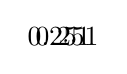
\begin{tikzpicture}
                \node[inner sep=0] at (0,0){\mygrid{0.25}{1}};
                \node[inner sep=0] at (-.1,0){\mygrid{0.25}{1}};
            \end{tikzpicture}
            };

            \node[net,right=of minus] (resnet) {ResNet};
            \node[right=of resnet] (h0) {\mygrid{0.25}{1}};
            
            \node[net, right=of h0, align=left] (h1) {PSP\\Module};
            \node[h, right=of h1] (h2) {
                %\mygrid{0.125}{1}
                \includegraphics[width=1.2cm]{\labelimage}
            };
            
            %\draw[shared]  (resnetpost) -- (resnetpre) node[midway, left]{\tiny $\textbf{W}$};

            \draw[conn] (inputpre.east)++(0,1em) -| (minus);
            \draw[conn] (inputpost.east)++(0,-1em) -| (minus);
            \draw[conn] (minus) -- (resnet);
            \draw[conn] (resnet) -- (h0);
            \draw[conn] (h0) -- (h1);
            \draw[conn] (h1) -- (h2);

		}
	}
}



\tikzset{pic shift/.store in=\shiftcoord,
	pic shift={(0,0)},
	pics/s2damagenetold/.style={
		code={

            \coordinate (center) at (0,0);
            
            % \includegraphics[width=2cm]{\vhrimage} 
            \node[above=-.4em of center, label={[label distance=0em, rotate=0]left:\small pre}] (inputpre) {\myimage{width=1.2cm}{\preimage}};
            \node[net,right=of inputpre] (resnetpre) {ResNet};
            \node[right=of resnetpre] (h0pre) {\mygrid{0.25}{1}};
            
            \node[below=-.4em of center, label={[label distance=0em, rotate=0]left:\small post}] (inputpost) {\myimage{width=1.2cm}{\postimage}};
            \node[net,right=of inputpost] (resnetpost) {ResNet};
            \node[right=of resnetpost] (h0post) {\mygrid{0.25}{1}};
            
            \coordinate (centerend) at ($ (h0pre.east)!0.5!(h0post.east) $);
            
            \node[right=of centerend] (minus) {
            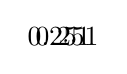
\begin{tikzpicture}
                \node[inner sep=0] at (0,0){\mygrid{0.25}{1}};
                \node[inner sep=0] at (.1,0){\mygrid{0.25}{1}};
            \end{tikzpicture}
            };
            
            \node[h, right=of minus] (h1) {\mygrid{0.125}{1}};
            \node[h, right=of h1] (h2) {\mygrid{0.125}{1}};
            
            \draw[shared]  (resnetpost) -- (resnetpre) node[midway, left]{\tiny $\textbf{W}$};

            \draw[conn] (inputpre) -- (resnetpre);
            \draw[conn] (resnetpre) -- (h0pre);
            \draw[conn] (h0pre) -| (minus);
            \draw[conn] (inputpost) -- (resnetpost);
            \draw[conn] (resnetpost) -- (h0post);
            \draw[conn] (h0post) -| (minus);
            
            \draw[conn] (minus) -- (h1);
            \draw[conn] (h1) -- (h2);

		}
	}
}

\newcommand{\figpspmodule}{
    \begin{tikzpicture}[node distance=.5em]
    
    \begin{scope}[xscale=1.5, yscale=-1.25]
    
    \node(pool) at (-1.2,2.1) {pool};
    %\node(upsample) at (3.5,1.5) {upsample};
    
    \node[grid](grid1) at (0,0){\mygridd{.3}{.5}{.5}};
    \node[grid](grid2) at (0,.8){\mygridd{.5}{.5}{.25}};
    \node[grid](grid3) at (0,1.8){\mygridd{.75}{.5}{.25}};
    \node[grid](grid16) at (0,3){\mygridd{1}{.5}{.25}};
    
    \coordinate[below right= 1em and 2em of grid16](convcoord);
    
    \node(conv1) at (1,0) {conv};
    \node(conv2) at (1,.8) {conv};
    \node(conv3) at (1,1.8) {conv};
    \node(conv16) at (1,3) {conv};
    
    \node[grid](gridd1) at (2,0){\mygridd{.3}{.2}{.5}};
    \node[grid](gridd2) at (2,.8){\mygridd{.5}{.2}{.25}};
    \node[grid](gridd3) at (2,1.8){\mygridd{.75}{.2}{.25}};
    \node[grid](gridd16) at (2,3){\mygridd{1}{.2}{.25}};
    
    \end{scope}
    
    \draw[conn] (pool) -- ++(2em,0) |- (grid1);
    \draw[conn] (pool) -- ++(2em,0) |- (grid2);
    \draw[conn] (pool) -- ++(2em,0) |- (grid3);
    \draw[conn] (pool) -- ++(2em,0) |- (grid16);
    
    \draw[conn] (grid1) -- (conv1) -- (gridd1);
    \draw[conn] (grid2) -- (conv2) -- (gridd2);
    \draw[conn] (grid3) -- (conv3) -- (gridd3);
    \draw[conn] (grid16) -- (conv16) -- (gridd16);
    
    %\draw[conn] (gridd1) -- ++(2em,0) |- (upsample);
    %\draw[conn] (gridd2) -- ++(2em,0) |- (upsample);
    %\draw[conn] (gridd3) -- ++(2em,0) |- (upsample);
    %\draw[conn] (gridd16) -- ++(2em,0) |- (upsample);
    
    \node[draw, rounded corners, label={[align=center]below:Pyramid Spatial Pooling (PSP) \\ Module}, fit=(pool)(grid1)(gridd16)]{};
    
    %\node[right=of upsample]{\mygridfour{1}{.2}{.25}};
    
    \end{tikzpicture}
}
%
%\begin{tikzpicture}[node distance=.75em, scale=1]
%
%\def\vhrimage{images/tile/vhr}
%\def\labelimage{images/tile/flooded}
%\def\labelimage{images/tile/buildings}
%\draw pic (base) at (0,0) {vhrbaseline};
%
%\def\preimage{images/tile/coh_int_20170706_20170823}
%\def\postimage{images/tile/coh_int_20170823_20170904}
%\draw pic (s2damagenet) at (0,2.1) {s2damagenet};
%%\coordinate (c1) at ($ (s2damageneth2)!0.5!(baseh3) $);
%%\draw[conn] (s2damageneth2) -| ($ (baseh3.north) + (-.2em,0) $);
%
%\def\preimage{images/tile/s2pre}
%\def\postimage{images/tile/s2post}
%\draw pic (s2damagenetsar) at (0,4.7) {s2damagenet};
%%\draw[conn] (s2damagenetsarh2) -| ($ (baseh3.north) + (.2em,0) $);
%
%\node[right=3em of s2damageneth2](out){\includegraphics[width=1.2cm]{images/tile/buildings}};
%
%\draw[conn] (s2damageneth2) -- (out);
%\draw[conn] (s2damagenetsarh2) -| ($ (s2damagenetsarh2.east)!0.5!(out.west) $) |- (out.west);
%\draw[conn] (basepspout) -| ($ (basepspout.east)!0.5!(out.west) $) |- (out.west);
%
%\end{tikzpicture}


\end{frame}

\begin{frame}
\frametitle{Publications and Code}



\textbf{AAAI 2019 Conference Paper:}

{\small
Rudner, T. G., Rußwurm, M., Fil, J., Pelich, R., Bischke, B., Kopackova, V., \& Bilinski, P. (2019). Multi $^{\mathbf {3}} $ Net: Segmenting Flooded Buildings via Fusion of Multiresolution, Multisensor, and Multitemporal Satellite Imagery. Association for the Advancement of Artificial Intelligence AAAI-19.}

\vspace{2em}

\textbf{2 NeurIPS Workshop Papers} at \textbf{AI for Social Good} and \textbf{Spatio-Temporal Workshops}.

%\vspace{1em}
%
%\textbf{NeurIPS18 Spatio-Temporal Workshop:}\\
%{\small
%Fil, J., Rudner, T. G., Russwurm, M., Bischke, B., Pelich, R., Kopackova, V., \& Bilinski, P. (2018). Multi³Net: Segmenting Flooded Buildings via Fusion of Multiresolution, Multisensor, and Multitemporal Satellite Imagery. NeurIPS18 Spatio-Temporal Workshop}
%
%\vspace{1em}
%
%\textbf{NeurIPS18 AI for Social Good Workshop:}\\
%{\small
%Rudner, T. G., Rußwurm, M., Fil, J., Pelich, R., Bischke, B., \& Kopacková, V. Rapid Computer Vision-Aided Disaster Response via Fusion of Multiresolution, Multisensor, and Multitemporal Satellite Imagery. NeurIPS18 AI for Social Good Workshop.
%}

\vspace{1em}
\textbf{GitHub}
\url{https://github.com/FrontierDevelopmentLab/multi3net}

\end{frame}

\begin{frame}[t]
	\frametitle{Workshops}
	
	\begin{columns}[t]
		
		\column{.5\textwidth}
		\textbf{CVPR EarthVision}
		\vspace{1em}
		
		\includegraphics[width=\textwidth]{images/EarthVision}
		
		Workshop CVPR \textbf{June 17, 2019}
		\url{https://www.grss-ieee.org/earthvision2019/}
		
		\column{.5\textwidth}
		\textbf{ECML MACLEAN}
		\vspace{1em}
	
		\includegraphics[width=\textwidth]{images/maclean-1-768x245}
		
		\vspace{3em}
		
		Deadline \textbf{Deadline June 10th, 2019}
		
		Workshop ECML \textbf{September 20th, 2019}
		
	
	\end{columns}
\end{frame}

%\begin{frame}
%	\frametitle{Summing Up}
%	
%	
%\end{frame}

%
%\begin{frame}
%\frametitle{CVPR EarthVision}
%
%\begin{columns}[t]
%	\column{.25\textwidth}
%		Long Beach, USA
%		
%		\textbf{Deadline passed}
%		
%		Workshop CVPR \textbf{June 17, 2019}
%		
%		\url{https://www.grss-ieee.org/earthvision2019/}
%	\column{.75\textwidth}
%	
%		\includegraphics[width=\textwidth]{images/EarthVision}
%		
%		Deadline \textbf{June 10th, 2019}
%		
%		Workshop ECML \textbf{September 20th, 2019}
%		
%	
%\end{columns}
%\end{frame}
%
%\begin{frame}
%	\frametitle{ECML MACLEAN}
%
%	\begin{columns}[t]
%		\column{.25\textwidth}
%		
%		Würzburg Germany
%		
%		Deadline \textbf{Deadline June 10th, 2019}
%		
%		Workshop ECML \textbf{September 20th, 2019}
%	
%		
%		\url{https://mdl4eo.irstea.fr/maclean-machine-learning-for-earth-observation/}
%		
%		\column{.75\textwidth}
%		
%		\includegraphics[width=\textwidth]{images/maclean-1-768x245}
%		
%	\end{columns}
%
%\end{frame}
%	
%	Earth observation and Machine Learning workshop at ECML/PKDD 
%	\url{http://ecmlpkdd2019.org/}


\begin{frame}
\frametitle{Summary}

\begin{columns}
	
	\column{.5\textwidth}
	
	\visible<1->{
		\textbf{Earth Observation}
		\begin{itemize}
			\item general overview on optical data
			\item complexity of Earth Observation data
			\item showed the balance between \textbf{spatial}, \textbf{temporal} and \textbf{spectral} resolution
		\end{itemize}
	}
	
	\visible<2->{
		\textbf{Projects}
		\begin{itemize}
			\item illustrated some ML-related tasks
%			\item outlined some challenges associated with EO
			\item translate methods between disciplines		
			\item connect via huge Benchmark Datasets	
		\end{itemize}
	}
	
	\visible<3->{
		\textbf{Initiatives}
		\begin{itemize}
			\item hope to \textbf{see you at one of the Workshops}
			\item or at \textbf{Frontier Developments Lab}!
		\end{itemize}
	}
	
	\column{.5\textwidth}
	
	\includegraphics[width=7cm]{images/dscovrepic/epicw1}
	
\end{columns}

\end{frame}

{\setbeamercolor{background canvas}{bg=black}
	\begin{frame}[plain]
	\vfill
	\begin{center}
		\Huge\color{tumwhite}
		\only<1>{
			\textbf{Thank you!}
			\includegraphics[width=6cm]{images/Bavaria_sat}
		}
		\only<2>{
			\textbf{Questions/Input?}
			\includegraphics[width=7cm]{images/France_white}
		}
%		\only<3>{
%			\textbf{Collaborations?}
%			\includegraphics[width=7cm]{images/France_white}
%		}
%		
	\end{center}


\vspace{1em}	
\color{tumbluelight}
\textbf{Twitter}: @marccoru | \textbf{Github}: @marccoru or @tum-lmf | \textbf{Chair} \url{lmf.bgu.tum.de/vision} \\ 

\vspace{1em}

\Large
BreizhCrops \url{https://github.com/TUM-LMF/BreizhCrops}
	
\vfill
\end{frame}
}


\begin{frame}
	\frametitle{Thank you!}
	
	\small
	
	\textbf{Papers:}
	\begin{columns}[t]
		
		\column{.5\textwidth}
		
		\begin{itemize}
			\item Rußwurm, M. and Körner, M. (2017). \textbf{Temporal Vegetation Modelling using Long Short-Term Memory Networks for Crop Identification from Medium-Resolution Multi-Spectral Satellite Images}. In IEEE/ISPRS EarthVision 2017 Workshop, Proceedings of the IEEE CVPR Workshops. \textbf{\color{tumorange} Best Paper Award}
			\item 	Rußwurm, M., Lefèvre, S., Courty, N., Emonet, R., Körner, M., \& Tavenard, R. (2019).\textbf{ End-to-end Learning for Early Classification of Time Series}. arXiv preprint arXiv:1901.10681.
			\item Rußwurm, M., \& Körner, M. (2018). \textbf{Multi-temporal land cover classification with sequential recurrent encoders}. ISPRS International Journal of Geo-Information, 7(4), 129.
		\end{itemize}
		
		\column{.5\textwidth}
		\begin{itemize}
			\item Rußwurm, M., \& Körner, M. (2018). \textbf{Convolutional LSTMs for Cloud-Robust Segmentation of Remote Sensing Imagery}. NeurIPS2018 Spatiotemporal Workshop. https://openreview.net/pdf?id=Sye7df9CK7
			\item Rudner, T. G. J.; Rußwurm, M.; Fil, J.; Pelich, R.; Bischke, B.; Kopačková, V.; Biliński, P. (2019) \textbf{Segmenting Flooded Buildings via Fusion of Multiresolution, Multisensor, and Multitemporal Satellite Imagery}. In AAAI.
		\end{itemize}
		
		\normalsize
		
		\vspace{1em}		
		\textbf{Twitter}
		\begin{itemize}
			\item https://twitter.com/MarcCoru
		\end{itemize}
		
		\textbf{Github}
		\begin{itemize}
			\item https://github.com/marccoru
			\item https://github.com/TUM-LMF
		\end{itemize}
		
	\end{columns}
\end{frame}


\addtocounter{framenumber}{-8}

\begin{frame}
\frametitle{Our Agenda}
\large 

\begin{columns}[t]
	\column{.5\textwidth}
	use pure \textbf<1>{data-driven end-to-end} learning
	\begin{itemize}
		\item no pre/postprocessing of data
		\item top-of-atmosphere data
		\item no atmospheric correction
		\item no cloud filtering
		\item no additional image registration
	\end{itemize}
	\vspace{1em}
	adapt established methods to EO Sensors
	\begin{itemize}
		\item NLP to EO: Sentence translation to image sequence classification
	\end{itemize}
	
	\column{.5\textwidth}
	\vspace{-2em}
	\uncover<1->{
		\centering 
		
\tikzsetnextfilename{datenbasiert}

% exclude this file from externalize otherwise the if else condition dies not work
\tikzset{external/export=false}
\begin{tikzpicture}[]

% if drawdl the deep learning part is drawn
\providecommand{\drawdl}{1}

\def\size{1.5cm}
\def\iosize{1.5cm}

\tikzstyle{illustration}=[yshift=-5mm]
\tikzstyle{element}=[draw=tumivory, fill=white, inner sep=2mm, rounded corners, node distance=4em and 2em]
\tikzstyle{ioelement}=[draw=tumivory, fill=tumwhite, inner sep=2mm, rounded corners, node distance=4em and 2em]
\tikzstyle{edge}=[rounded corners=3mm]

\node[ioelement, align=center,label=above:{$\M{X}$}](input){\resizebox{\iosize}{!}{\begin{tikzpicture}
	% each layer
	
	% raster size
  \def\d{0.73}  	
	
	% distance layer
	\def\s{\d*5}
	
	\foreach \i in {1,...,6}
	{		
		\begin{scope}[
      yshift=\s*\i,every node/.append style={
			yslant=0.5,xslant=-1},yslant=0.5,xslant=-1
		]
		%\draw[step=3.33mm] (0,0) grid (1,1);
		%\fill[black,fill opacity=.9] (0.333,0.333) rectangle (0.333,0.333);    	    	  
		
		\foreach \row in {0,...,2}{
			\foreach \col in {0,...,2}{
				\draw[tumblack, fill=tumblue!\pdfuniformdeviate 40,fill opacity=1,rounded corners=1] (\col*\d/3,\row*\d/3) rectangle (\col*\d/3+\d/3, \row*\d/3+\d/3);
	        }
		}
		\end{scope}
	}	
\end{tikzpicture}}}; %input\\$\VInput \in \R^D$
%\node[illustration,above=of input](raster){};

\node[element, right = of input,label=below:{end-to-end learning}](eelearning){
	\hspace{-1em}\input{images/fcnet.tikz}
}; %\emph{end-to-end learning}

\node[ioelement,right=of eelearning, align=center,label=above:{$\V{y}$}](result){
	\resizebox{!}{\iosize}{
%		\rotatebox{90}{
			\tikz{
	\begin{scope}[rotate=90]
	%\draw[step=0.2] (0,0) grid (2,.2);
	\foreach \i in {0,...,6}
	\draw[tumblack,fill=tumorange!\pdfuniformdeviate 40,fill opacity=.9, rounded corners=0.5] (\i*.2,0) rectangle (\i*.2+.2,.2);
	%       \draw[black,fill=black!\pdfuniformdeviate 40,fill opacity=.9, rounded corners=0.5] (\i*.2,0) rectangle (\i*.2+.2,.2);
	
	\end{scope}
}
%		}
	}
};
%\node[illustration,above=of result](classprob){\resizebox{1cm}{!}{\vectorgrid}};


% arrows
\draw [-stealth, edge, draw=black] (input) -- (eelearning) -- (result);


\end{tikzpicture}

	}
	
	%			\vspace{1em}
	
	
\end{columns}

\end{frame}


\begin{frame}{UCR Datasets}

%	\begin{columns}
%		\column{.6\textwidth}
%		
\begin{itemize}[leftmargin=0cm]
	\item broad family of \textbf{46 diverse datasets}
	\item \textbf{accuracies reported} from other early classification approaches
	\item covers \textbf{sensor data}, \textbf{motion tracking}, \textbf{electrocardiography data}
	\item many, but \textbf{small datasets} \small{(overall circa 500 MB)}
\end{itemize}
%		\column{.4\textwidth}
%		\includegraphics[width=\textwidth]{images/UCR}
%	\end{columns}

\vspace{.5em}
\centering\includegraphics[width=5cm]{images/GunPoint}

\vspace{.5em}

{\small \texttt{http://www.timeseriesclassification.com/}
}
\end{frame}


\begin{frame}
\frametitle{Communications}
\centering
\begin{tikzpicture}[xscale=3.5, yscale=2]
%\draw[fill=tumblue, draw=none, opacity=0.5](-1,0) circle (1.5);
\node[fill=tumbluelight, draw=none, opacity=0.5, circle, minimum width=6cm, label=Earth Observation] at (-1,0){};

\node[fill=tumorange!50, draw=none, opacity=0.5, circle, minimum width=6cm, label=Machine Learning] at (1,0){};
%\draw[fill=tumorange, draw=none, opacity=0.5](1,0) circle (1.5);

%\node at (-1.3,1){Data};

\node[text width=3.5cm] at (-1,.9){\focusmethod is a \textbf{tool} for our \focusdata};
\node[text width=3.5cm] at (1,.9){\focusdata is a \textbf{benchmark} for our \focusmethod};


\node[text width=3.5cm] at (-1,.3){\textbf{should generalize} to applications of a \\ specific sub-field};
\node[text width=3.5cm] at (1,.3){\textbf{must generalize} to many fields of applications};

\node[text width=3.5cm] at (-1,-.3){data has specific \\ \textbf{phyisical properties}};
\node[text width=3.5cm] at (1,-.3){data is a \textbf{feature vector}};
%
%\node[text width=2cm] at (-1.3,-.6){{physics}, {sensors}, {applications}};

%\node at (1.3,1){Method};

%\node at (-1.3,1){IGARSS};
%\node at (-1.6,-1){ISPRS};
%\node at (-1.2,-.6){IEEE-GRSS};
%\node at (-1.8,.4){MDPI-RS Journal};
%\node at (-1.3,0){RSE Journal};
%
%\node at (1.3,1){NeurIPS};
%\node at (1.6,-1){CVPR};
%\node at (1.2,-.6){ICML};
%\node at (1.8,.4){ECCV};
%\node at (1.3,.2){ECML};
%
%\node at (0,.5){CVPR EarthVision};
%\node at (0,0){ECML MACLEAN};
%\node at (0,-.5){(ESA-$\Phi$-week)};

\end{tikzpicture}

\end{frame}

\begin{frame}<presentation:3>
\frametitle{Chair of Remote Sensing Technology}


    \resizebox{\linewidth}{!}{
      \begin{tikzpicture}[scale=.75,font=\scriptsize,draw=tumblue]
        
        % university
        \draw[draw,fill=tumbluelight] (0,0) rectangle node{Technical University of Munich} +(9, 1);
        \draw[draw=none,fill=none] (0.25,.01) rectangle node{\includegraphics[width=1cm]{images/logo-blue-TUM.pdf}} +(1,1);
        
        % faculty
        \draw[draw] (0,1) rectangle node{} +(1,1);
        \draw[draw=none] (1,1) rectangle node{\ldots} +(1,1);
        \draw[draw, fill=tumbluelight!75] (2,1) rectangle node[align=center]{Faculty of Geo, Civil and\\ Environmental Engineering} +(7,1);

        % groups
        \draw[draw] (2,2) rectangle node{} +(1,3);
        \draw[draw=none] (3,2) rectangle node{\ldots} +(1,3);

        \draw[draw] (4,5) rectangle node[align=center, font=\tiny]{Prof.\\U. Stilla} +(1.5,1);
        \draw[draw] (4,2) rectangle node[align=center, anchor=base, yshift=-1mm, font=\tiny]{\emph{FPF}\\[1mm]Photo-\\grammetry\\and Remote\\Sensing} +(1.5,3);
        
        \visible<5->{%
          \draw[draw, fill=tumbluelight!25] (5.5,5) rectangle node[align=center, font=\tiny, name=SiPEO_XZ]{Prof.\\X. Zhu} +(1.5,1);
          \draw[draw, fill=tumbluelight!25] (5.5,2) rectangle node[align=center, anchor=base, yshift=-1mm, font=\tiny]{%
            \emph{SiPEO}\\[1mm]Signal\\Processing\\in Earth\\Observation
          } +(1.5,3);
        }
        
        \visible<2->{%
          \draw[draw, fill=tumbluelight!50] (7,5) rectangle node[align=center, font=\scriptsize\bf, name=LMF_RB] {Prof.\\R. Bamler} +(2,1);
          \draw[draw, fill=tumbluelight!50] (7,2) rectangle node[align=center, anchor=base, yshift=-1mm, font=\tiny]{%
            \emph{LMF}\\[1mm]Chair of \\Remote\\Sensing\\Technology
          } +(2,3);
        }

        
        \visible<3->{%
          \draw[draw=tumgreen, fill=tumgreen!50, rounded corners=3pt] (7.1,2.1) rectangle node[align=center, font=\tiny]{Computer Vision\\Research Group\\[1mm]Dr. M. Körner} +(1.8,1);
        }


        \visible<4->{%
          \draw[draw=tumorange, fill=tumorange!50] (10,1) rectangle node[align=center]{Remote Sensing Technology Institute \textit{(IMF)}} +(7.5,1);
          \draw[draw=none] (17.25,1) rectangle node{\ldots} +(1,1);
          \draw[draw=tumorange] (18,1) rectangle node{} +(1,1);

          \draw[draw=tumorange, fill=tumorange!75] (10,0) rectangle node[align=center]{German Aerospace Center\\Campus Oberpfaffenhofen near Munich} +(9, 1);
          \draw[draw=none,fill=none] (17.5,.01) rectangle node{\includegraphics[height=.6cm]{images/logo-black-DLR}} +(1,1);

          \draw[draw=tumorange, fill=tumorange!25] (10,2) rectangle node[align=center, font=\tiny]{Photo-\\grammetry\\ and\\Image\\Analysis} +(1.5,2);
          \draw[draw=tumorange, fill=tumorange!25] (10,4) rectangle node[align=center, font=\tiny]{Prof.\\P. Reinartz} +(1.5,1);

          \draw[draw=tumorange, fill=tumorange!25] (11.5,2) rectangle node[align=center, font=\tiny]{SAR\\Signal\\Processing} +(1.5,2);
          \draw[draw=tumorange, fill=tumorange!25] (11.5,4) rectangle node[align=center, font=\tiny]{Prof.\\M. Eineder} +(1.5,1);

          \draw[draw=tumorange, fill=tumorange!25] (13.0,2) rectangle node[align=center, font=\tiny]{Atmospheric\\ Processors} +(1.5,2);
          \draw[draw=tumorange, fill=tumorange!25] (13.0,4) rectangle node[align=center, font=\tiny]{Prof.\\T. Trautmann} +(1.5,1);

          \draw[draw=tumorange, fill=tumorange!25] (14.50,2) rectangle node[align=center, font=\tiny]{Experimental\\ Methods} +(1.5,2);
          \draw[draw=tumorange, fill=tumorange!25] (14.50,4) rectangle node[align=center, font=\tiny]{Prof. P. \\Haschberger} +(1.5,1);

%          \visible<5->{%
            \draw[draw=tumorange, fill=tumorange!25] (16.00,2) rectangle node[align=center, font=\tiny]{Data Science\\ in Earth\\ Observation} +(1.5,2);
            \draw[draw=tumorange, fill=tumorange!25] (16.00,4) rectangle node[align=center, font=\tiny, name=DAS_XZ]{Prof.\\ X. Zhu} +(1.5,1);
%          }

          \draw[draw=tumorange, fill=tumorange!25] (10,5) rectangle node[align=center, font=\scriptsize\bf]{Prof. R. Bamler} +(7.5,1) ;


        %   \draw[draw=none, shade, left color=tumbluelight, right color=tumorange!25] (9,2) rectangle node{} +(1,4);
          \fill[draw=none, draw opacity=0, shade, left color=tumbluelight!50, right color=tumorange!25] (9,2) -- (9,6) -- (10,6) -- (10,1) -- cycle;
          \draw[stealth-stealth] (9,5.5) -- (10,5.5) ;
        
%           \draw[stealth-stealth] (SiPEO_XZ.north) |- +(0,1) -| (DAS_XZ.north) +(-1,0);
        }

      \end{tikzpicture}
    }
\end{frame}

\begin{frame}<presentation:5>
\frametitle{Chair of Remote Sensing Technology}


    \resizebox{\linewidth}{!}{
      \begin{tikzpicture}[scale=.75,font=\scriptsize,draw=tumblue]
        
        % university
        \draw[draw,fill=tumbluelight] (0,0) rectangle node{Technical University of Munich} +(9, 1);
        \draw[draw=none,fill=none] (0.25,.01) rectangle node{\includegraphics[width=1cm]{images/logo-blue-TUM.pdf}} +(1,1);
        
        % faculty
        \draw[draw] (0,1) rectangle node{} +(1,1);
        \draw[draw=none] (1,1) rectangle node{\ldots} +(1,1);
        \draw[draw, fill=tumbluelight!75] (2,1) rectangle node[align=center]{Faculty of Geo, Civil and\\ Environmental Engineering} +(7,1);

        % groups
        \draw[draw] (2,2) rectangle node{} +(1,3);
        \draw[draw=none] (3,2) rectangle node{\ldots} +(1,3);

        \draw[draw] (4,5) rectangle node[align=center, font=\tiny]{Prof.\\U. Stilla} +(1.5,1);
        \draw[draw] (4,2) rectangle node[align=center, anchor=base, yshift=-1mm, font=\tiny]{\emph{FPF}\\[1mm]Photo-\\grammetry\\and Remote\\Sensing} +(1.5,3);
        
        \visible<5->{%
          \draw[draw, fill=tumbluelight!25] (5.5,5) rectangle node[align=center, font=\tiny, name=SiPEO_XZ]{Prof.\\X. Zhu} +(1.5,1);
          \draw[draw, fill=tumbluelight!25] (5.5,2) rectangle node[align=center, anchor=base, yshift=-1mm, font=\tiny]{%
            \emph{SiPEO}\\[1mm]Signal\\Processing\\in Earth\\Observation
          } +(1.5,3);
        }
        
        \visible<2->{%
          \draw[draw, fill=tumbluelight!50] (7,5) rectangle node[align=center, font=\scriptsize\bf, name=LMF_RB] {Prof.\\R. Bamler} +(2,1);
          \draw[draw, fill=tumbluelight!50] (7,2) rectangle node[align=center, anchor=base, yshift=-1mm, font=\tiny]{%
            \emph{LMF}\\[1mm]Chair of \\Remote\\Sensing\\Technology
          } +(2,3);
        }

        
        \visible<3->{%
          \draw[draw=tumgreen, fill=tumgreen!50, rounded corners=3pt] (7.1,2.1) rectangle node[align=center, font=\tiny]{Computer Vision\\Research Group\\[1mm]Dr. M. Körner} +(1.8,1);
        }


        \visible<4->{%
          \draw[draw=tumorange, fill=tumorange!50] (10,1) rectangle node[align=center]{Remote Sensing Technology Institute \textit{(IMF)}} +(7.5,1);
          \draw[draw=none] (17.25,1) rectangle node{\ldots} +(1,1);
          \draw[draw=tumorange] (18,1) rectangle node{} +(1,1);

          \draw[draw=tumorange, fill=tumorange!75] (10,0) rectangle node[align=center]{German Aerospace Center\\Campus Oberpfaffenhofen near Munich} +(9, 1);
          \draw[draw=none,fill=none] (17.5,.01) rectangle node{\includegraphics[height=.6cm]{images/logo-black-DLR}} +(1,1);

          \draw[draw=tumorange, fill=tumorange!25] (10,2) rectangle node[align=center, font=\tiny]{Photo-\\grammetry\\ and\\Image\\Analysis} +(1.5,2);
          \draw[draw=tumorange, fill=tumorange!25] (10,4) rectangle node[align=center, font=\tiny]{Prof.\\P. Reinartz} +(1.5,1);

          \draw[draw=tumorange, fill=tumorange!25] (11.5,2) rectangle node[align=center, font=\tiny]{SAR\\Signal\\Processing} +(1.5,2);
          \draw[draw=tumorange, fill=tumorange!25] (11.5,4) rectangle node[align=center, font=\tiny]{Prof.\\M. Eineder} +(1.5,1);

          \draw[draw=tumorange, fill=tumorange!25] (13.0,2) rectangle node[align=center, font=\tiny]{Atmospheric\\ Processors} +(1.5,2);
          \draw[draw=tumorange, fill=tumorange!25] (13.0,4) rectangle node[align=center, font=\tiny]{Prof.\\T. Trautmann} +(1.5,1);

          \draw[draw=tumorange, fill=tumorange!25] (14.50,2) rectangle node[align=center, font=\tiny]{Experimental\\ Methods} +(1.5,2);
          \draw[draw=tumorange, fill=tumorange!25] (14.50,4) rectangle node[align=center, font=\tiny]{Prof. P. \\Haschberger} +(1.5,1);

%          \visible<5->{%
            \draw[draw=tumorange, fill=tumorange!25] (16.00,2) rectangle node[align=center, font=\tiny]{Data Science\\ in Earth\\ Observation} +(1.5,2);
            \draw[draw=tumorange, fill=tumorange!25] (16.00,4) rectangle node[align=center, font=\tiny, name=DAS_XZ]{Prof.\\ X. Zhu} +(1.5,1);
%          }

          \draw[draw=tumorange, fill=tumorange!25] (10,5) rectangle node[align=center, font=\scriptsize\bf]{Prof. R. Bamler} +(7.5,1) ;


        %   \draw[draw=none, shade, left color=tumbluelight, right color=tumorange!25] (9,2) rectangle node{} +(1,4);
          \fill[draw=none, draw opacity=0, shade, left color=tumbluelight!50, right color=tumorange!25] (9,2) -- (9,6) -- (10,6) -- (10,1) -- cycle;
          \draw[stealth-stealth] (9,5.5) -- (10,5.5) ;
        
%           \draw[stealth-stealth] (SiPEO_XZ.north) |- +(0,1) -| (DAS_XZ.north) +(-1,0);
        }

      \end{tikzpicture}
    }
\end{frame}


\begin{frame}
\frametitle{Summary: Balancing Resolutions}

\begin{columns}
	\column{.5\textwidth}


\begin{tikzpicture}[scale=3,
x={(\raarot cm,\rbarot cm)},%
y={(\rabrot cm, \rbbrot cm)},%
z={(\racrot cm, \rbcrot cm)}]




\draw [->] (0,0,0) -- (1.2,0,0) node[anchor=north east]{spatial};
\draw [->] (0,0,0) -- (0,1.2,0) node[anchor=north west]{spectral};
\draw [->] (0,0,0) -- (0,0,1.2) node[anchor=south]{temporal};   

\draw (0,0,1) node[right] {hours};
\draw (0,0,0.66) node[right] {days};
\draw (0,0,0.33) node[right] {weeks};

\draw (0,.33,0) node[right] {3};
\draw (0,.66,0) node[right] {15};
\draw (0,1,0) node[right] {$>$100};

\draw (1,0,0) node[above left] {$<$1m};
\draw (.8,0,0) node[above left] {10m};
\draw (.6,0,0) node[above left] {100m};
\draw (.4,0,0) node[above left] {1km};
\draw (.2,0,0) node[above left] {10km};


%% High Resolution
\visible<2>{\domain{1.2}{0.4}{.6}{tumgreen};}

%% environmental satellites
\visible<3>{\domain{0.5}{.9}{.9}{tumorange};}

%% Hyper-spectral
\visible<4>{\domain{0.7}{1.3}{.2}{tumgreen};}

%% Multi-spectral
\visible<5>{\domain{0.9}{.7}{.7}{tumgreen};}

%% weather satellites	
\visible<6>{\domain{0.3}{.6}{1.2}{tumblue};}

\end{tikzpicture}

\column{.5\textwidth}

\visible<2->{
	\textbf{Scheduled Acquisitions}
	\begin{itemize}
		\item<2-> very high spatial Resolution Imagery
	\end{itemize}
}
\visible<3->{
	\textbf{Global coverage and open data policy}
	\begin{itemize}
		\item<3-> multi-spectral satellites
		\item<4-> environmental satellites
		\item<5-> weather satellites
	\end{itemize}
	
}

\end{columns}
\end{frame}


\begin{frame}
\frametitle{Augmenting Classification Models}

\begin{columns}
	
	\column{.5\textwidth}
	\begin{center}
		
		\input{images/backprop_example.tikz}
	\end{center}
	\column{.5\textwidth}
	\input{images/qualitative_example.tikz}
	
	
\end{columns}

\end{frame}



\begin{frame}
\frametitle{Earliness-Aware Loss function}

\Large

\begin{equation*}
\mathcal{L} = P(t)\left(\alpha (1-\yhat^+) + \left(1-\alpha\right) \frac{t}{T}\right)
\end{equation*}
\end{frame}


\begin{frame}
\frametitle{Spectral Bands}

\begin{columns}
	%	\column{.2\textwidth}
	%	
	%	\begin{equation*}
	%	\rho_{\lambda} = \int_{\lambda-\frac{b}{2}}^{\lambda-\frac{b}{2}} \rho_(\lambda) d\lambda
	%	\end{equation*}
	%	
	%	\vspace{1em}
	%	
	%	integrated between in spectral \textbf{bands} bounds $\lambda - \frac{b}{2}$ and $\lambda + \frac{b}{2}$ with the \emph{bandwidth} b.
	%	
	
	\column{.9\textwidth}
	
	\includegraphics[width=\textwidth]{images/Meer14Satellitebands}
	
	
\end{columns}

\vspace{1em}
{\small
	Van der Meer, F. D., Van der Werff, H. M. A., \& Van Ruitenbeek, F. J. A. (2014). Potential of ESA's Sentinel-2 for geological applications. Remote sensing of environment, 148, 124-133.
}

\end{frame}


\begin{frame}{Benchmark Datasets}

%	\begin{columns}
%		\column{.6\textwidth}
%		
\begin{itemize}[leftmargin=0cm]
	\item broad family of \textbf{46 diverse datasets}
	\item \textbf{accuracies reported} from other early classification approaches
	\item covers \textbf{sensor data}, \textbf{motion tracking}, \textbf{electrocardiography data}
	\item many, but \textbf{small datasets} \small{(overall circa 500 MB)}
\end{itemize}
%		\column{.4\textwidth}
%		\includegraphics[width=\textwidth]{images/UCR}
%	\end{columns}

{\textbf{GunPoint} dataset}
\vspace{.5em}
\centering\includegraphics[width=7cm]{images/GunPoint}

\vspace{.5em}

{\small \texttt{http://www.timeseriesclassification.com/}
}
\end{frame}

\begin{frame}
\frametitle{Two Fields}
\centering
\begin{tikzpicture}[scale=2]
%\draw[fill=tumblue, draw=none, opacity=0.5](-1,0) circle (1.5);
\node[fill=tumbluelight, draw=none, opacity=0.5, circle, minimum width=6cm, label=Earth Observation] at (-1,0){};

\node[fill=tumorange!50, draw=none, opacity=0.5, circle, minimum width=6cm, label=Machine Learning] at (1,0){};
%\draw[fill=tumorange, draw=none, opacity=0.5](1,0) circle (1.5);

\draw[-stealth, shorten >=1cm] (-1.3,1) -- (0,0);
\draw[-stealth, shorten >=1cm] (-1.6,-1) -- (0,0);
\draw[-stealth, shorten >=1cm] (-1.2,-.6) -- (0,0);
\draw[-stealth, shorten >=1cm] (-1.8,.4) -- (0,0);
\draw[-stealth, shorten >=1cm] (-1.3,.2) -- (0,0);

\node[font=\bfseries] at (-2,0) {applications};

\draw[-stealth, shorten >=1cm] (1.3,1) -- (0,0);
\draw[-stealth, shorten >=1cm] (1.6,-1) -- (0,0);
\draw[-stealth, shorten >=1cm] (1.2,-.6) -- (0,0);
\draw[-stealth, shorten >=1cm] (1.8,.4) -- (0,0);
\draw[-stealth, shorten >=1cm] (1.3,.2) -- (0,0);

\node[font=\bfseries] at (2,0) {methods};

%\node[text width=2cm, circle, fill=tumblue, text=white]{global scale};
%
%\node[text width=2cm, circle, fill=tumblue, text=white]{global scale};

%\node[font=\normalsize, fill=white, text width=2cm, rounded corners, fill opacity=.5, text opacity=1](phd) at (0,0){global scaleability \\ real world impact \\ Open Data};

%\draw[-stealth, very thick] (phd) -- (0,, fil0);
\end{tikzpicture}


\end{frame}


\begin{frame}
\frametitle{Communities}
\centering
\begin{tikzpicture}[scale=2]
%\draw[fill=tumblue, draw=none, opacity=0.5](-1,0) circle (1.5);
\node[fill=tumbluelight, draw=none, opacity=0.5, circle, minimum width=6cm, label=Earth Observation] at (-1,0){};

\node[fill=tumorange!50, draw=none, opacity=0.5, circle, minimum width=6cm, label=Machine Learning] at (1,0){};
%\draw[fill=tumorange, draw=none, opacity=0.5](1,0) circle (1.5);

\node at (-1.3,1){IGARSS};
\node at (-1.6,-1){ISPRS};
\node at (-1.2,-.6){IEEE-GRSS};
\node at (-1.8,.4){MDPI-RS Journal};
\node at (-1.3,0){RSE Journal};

\node at (1.3,1){NeurIPS};
\node at (1.6,-1){CVPR};
\node at (1.2,-.6){ICML};
%\node at (1.8,.4){ECCV};
\node at (1.5,.3){AISTATS};
%\node at (1.3,.2){ECML};
\node at (1.3,-.2){ICLR};

\node at (0,.5){CVPR EarthVision};
\node at (0,0){ECML MACLEAN};
\node at (0,-.5){(ESA-$\Phi$-week)};

\end{tikzpicture}
\end{frame}


\begin{frame}
\frametitle{MODIS Satellite}
\only<1>{\includegraphics[width=\textwidth]{images/modis/MODIS_UK}}
\only<2>{\includegraphics[width=\textwidth]{images/modis/MODIS_OXF}}
\end{frame}




%\begin{frame}
%\frametitle{References}
%% This prints the bibliography on the slide
%%\usepackage[backend=biber]{biblatex}
%\bibliography{bib/references.bib}
%\bibliographystyle{plain}
%% Removes icon in bibliography
%\setbeamertemplate{bibliography item}{}
%
%\end{frame}


\end{document}



